\documentclass[11pt]{article}
\usepackage[margin=1in]{geometry}
\usepackage{amsmath,amssymb,amsthm}
\usepackage{algorithm}
\usepackage{algpseudocode}
\usepackage{booktabs}
\usepackage{hyperref}
\usepackage{tikz}
\usetikzlibrary{arrows.meta}
\usepackage{graphicx}
\graphicspath{{figures/}}

\DeclareMathOperator{\argmax}{arg\,max}

\newtheorem{theorem}{Theorem}
\newtheorem{lemma}{Lemma}
\newtheorem{proposition}{Proposition}
\newtheorem{definition}{Definition}
\newtheorem{remark}{Remark}
\newtheorem{conjecture}{Conjecture}

\title{Certified Policy Bases for Successor-Feature Composition}
\author{}
\date{}

\begin{document}
\maketitle

\subsection*{Overview:}

\begin{center}
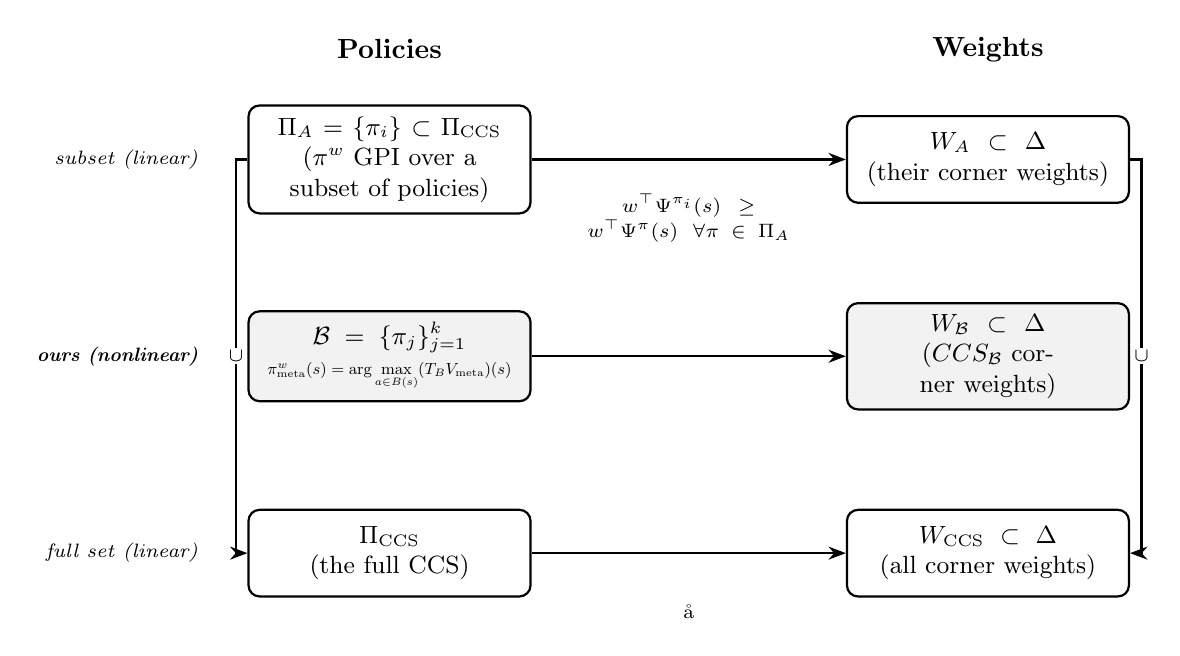
\begin{tikzpicture}[
    box/.style={draw, rounded corners, align=center, text width=3.3cm, minimum height=1.1cm, font=\small, inner sep=4pt},
    lbl/.style={font=\scriptsize, align=center, text width=3.6cm},
    tag/.style={font=\scriptsize\itshape},
    vlbl/.style={font=\scriptsize, align=center},
    >={Stealth[length=2.2mm]}, thick
]
    % column headers
    \node[font=\bfseries] (hpol) at (0,6.4) {Policies};
    \node[font=\bfseries] (hw)   at (7.6,6.4) {Weights};

    % row 1: a subset of policies
    \node[box] (p1) at (0,5) {$\Pi_A=\{\pi_i\}\subset\Pi_{\mathrm{CCS}}$\\($\pi^w$ GPI over a subset of policies)};
    \node[box] (w1) at (7.6,5) {$W_A\subset\Delta$\\(their corner weights)};
    \draw[->] (p1) -- (w1);
    \node[lbl] at (3.8,4.25) {$w^\top\Psi^{\pi_i}(s)\ge w^\top\Psi^{\pi}(s)\ \ \forall\pi\in\Pi_A$};
    \node[tag, anchor=east] at (-2.3,5) {subset (linear)};

    % row 2: ours
    \node[box, fill=black!5] (p2) at (0,2.5) {$\mathcal B=\{\pi_j\}_{j=1}^k$\\\resizebox{3.1cm}{!}{$\pi^w_{\mathrm{meta}}(s)=\arg\max\limits_{a\in B(s)}(T_BV_{\mathrm{meta}})(s)$}};
    \node[box, fill=black!5] (w2) at (7.6,2.5) {$W_{\mathcal B}\subset\Delta$\\($CCS_\mathcal{B}$ corner weights)};
    \draw[->] (p2) -- (w2);
    \node[tag, anchor=east] at (-2.3,2.5) {\textbf{ours (nonlinear)}};

    % row 3: full CCS
    \node[box] (p3) at (0,0) {$\Pi_{\mathrm{CCS}}$\\(the full CCS)};
    \node[box] (w3) at (7.6,0) {$W_{\mathrm{CCS}}\subset\Delta$\\(all corner weights)};
    \draw[->] (p3) -- (w3);
    \node[lbl] at (3.8,-0.75) {å};
    \node[tag, anchor=east] at (-2.3,0) {full set (linear)};

    % vertical union arrows, routed around row 2 via a side rail
    \draw[->] (p1.west) -- (-1.95,5) -- (-1.95,0) -- (p3.west);
    \node[vlbl, fill=white, inner sep=1pt] at (-1.95,2.5) {$\cup$};
    \draw[->] (w1.east) -- (9.55,5) -- (9.55,0) -- (w3.east);
    \node[vlbl, fill=white, inner sep=1pt] at (9.55,2.5) {$\cup$};
\end{tikzpicture}
\end{center}

In rows 1 and 3 the relation is linear in set union: $W_{A\cup B}=W_A\cup W_B$, so adding a policy only ever adds
its own corner weights, never changes anyone else's.

\pagebreak 

\section{Goals for a publication}

\begin{itemize}
  \item  Compute the CCS faster by using the combination of base and meta policies. Note, however, that it is not enough to get all the policies from the CCS, but it is more important to get the successor features to perform GPI correctly. 
  

  \item Provide an improved version of GPI, when the CCS is very big that we don't have time to compute all the policies, then perform GPI on a meta-policy particularly computed for that task. 
  
  \item Look how to implement it in Infante's paper. 
\end{itemize}

\pagebreak 

\section{Setup}\label{sec:setup}

A MO MDP  is $\mathcal{M}=(S,A,P,\phi,\gamma)$ with vector reward
$\phi:S\times A\to\mathbb{R}^d$. For a weight $w\in\Delta^{d-1}=\{w\ge0,\ || \mathbf{w} ||_1 =1\}$,
the scalarized reward is $\phi(s,a)^\top w$. The successor feature (SF) of policy $\pi$ is
\[
\Psi^\pi(s,a) = \mathbb{E}_\pi\Big[\textstyle\sum_{t\ge0}\gamma^t\phi(s_t,a_t)\ \Big|\ s_0=s,a_0=a\Big],
\qquad
\Psi^\pi(s,a)=\phi(s,a)+\gamma\,\mathbb{E}_{s'}\big[\Psi^\pi(s',\pi(s'))\big].
\]
$V^*_w(s)=\max_\pi \Psi^\pi(s,\pi(s))^\top w$ is the scalarized optimal value. The
\emph{convex coverage set} (CCS) is the set of SF vectors of policies optimal for some $w$;
recovering it is the standard multi-objective planning goal (Optimistic Linear Support, OLS).

\begin{definition}[Basis]
A \emph{basis} is a finite set $\mathcal{B}=\{(\pi_j,\Psi^{\pi_j})\}_{j=1}^k$ of exactly solved policies,
each $\pi_j$ optimal for its own training weight $w_j$: $\pi_j(s)=\arg\max_a \Psi^{\pi_j}(s,a)^\top w_j$.
Each $\pi_j$ is fixed once solved.
\end{definition}

\begin{definition}[Restricted MORL]\label{def:meta}
For a basis $\mathcal B$ and a state $s$, the restricted action set is exactly the base policies'
own actions,
\[
B(s) = \{\pi_1(s),\dots,\pi_k(s)\} \subseteq A(s), \qquad\text{i.e.}\quad a\in B(s) \iff a=\pi_j(s)\ \text{for some } j.
\]
For a query weight $w$, the restricted Bellman operator is
\[
(T_BV)(s)=\max_{a\in B(s)}\big[\phi(s,a)^\top w+\gamma\,\mathbb{E}_{s'}V(s')\big]
         =\max_{j\in\{1,\dots,k\}}\big[\phi(s,\pi_j(s))^\top w+\gamma\,\mathbb{E}_{s'}V(s')\big],
\]
a $\gamma$-contraction with unique fixed point
\[
V_{\mathrm{meta}}=T_BV_{\mathrm{meta}},
\]
We define a metapolicy over $\mathcal{B}$ as the greedy policy of this fixed point:
\[
\pi^w_{\mathrm{meta}}(s) \;=\; \pi_{j^*(s)}(s), \qquad
j^*(s) = \arg\max_{j\in\{1,\dots,k\}}\big[\phi(s,\pi_j(s))^\top w+\gamma\,\mathbb{E}_{s'}V_{\mathrm{meta}}(s')\big],
\]
\end{definition}

\begin{definition}[Bellman certificate]
For candidate value $V$ and weight $w$, the gap against the unrestricted operator $T$ is
\[
\mathrm{gap}_w(s;V) = (TV)(s)-V(s) = \max_{a\in A(s)}\big[\phi(s,a)^\top w+\gamma\,\mathbb{E}_{s'}V(s')\big]-V(s).
\]

Note that $\mathrm{gap}_w(s;V_{\mathrm{meta}})$ is always $\ge 0$ for any $s$ because $B(s) \subseteq A(s)$. If $\mathrm{gap}_w(s;V_{\mathrm{meta}})=0$ for all $s$, then $V_{\mathrm{meta}}=V^*_w$, and the metapolicy is optimal for that weight. 
\end{definition}


\begin{algorithm}[H]
\caption{\textsc{Certify-or-Grow}$(w,\mathcal{B})$}
\begin{algorithmic}[1]
\State $\pi_{\mathrm{meta}},\Psi^{\pi_{\mathrm{meta}}} \gets$ restricted policy iteration on $\mathcal B$ at $w$ \Comment{full table, not just $V_{\mathrm{meta}}$: one extra vector solve for the fixed greedy policy}
\State $V_{\mathrm{meta}}(\cdot)\gets\Psi^{\pi_{\mathrm{meta}}}(\cdot,\pi_{\mathrm{meta}}(\cdot))^\top w$
\If{$\max_s \mathrm{gap}_w(s;V_{\mathrm{meta}}) \le \mathrm{tol}$}
    \State \Return $\pi_{\mathrm{meta}},\ \Psi^{\pi_{\mathrm{meta}}},\ \mathcal{B}$
\Else
    \State $(\pi_w,\Psi^{\pi_w}) \gets$ unrestricted policy iteration at $w$ \label{alg:cog-fallback}
    \State $\mathcal{B}\gets\mathcal{B}\cup\{(\pi_w,\Psi^{\pi_w})\}$ \Comment{$\pi_w$ is trivially $\mathcal B$'s new metapolicy: gap $0$ by construction}
    \State \Return $\pi_w,\ \Psi^{\pi_w},\ \mathcal{B}$
\EndIf
\end{algorithmic}
\end{algorithm}

\subsection{How can we improve the GPI from base policies?}

The restricted metapolicy $\pi_{\mathrm{meta}}$ might not beat GPI, since GPI can also take actions no base policy
would ever take. We now motivate a policy that does at least as well. 

\begin{definition}[GPI estimate]
For a policy set $\Pi=\{\pi_1,\dots,\pi_k\}$ and weight $w$, $\widehat Q_\Pi(s,a) := \max_{j} \Psi^{\pi_j}(s,a)^\top w$,
and $\pi^{\mathrm{GPI}}_\Pi(s) := \arg\max_a \widehat Q_\Pi(s,a)$.
\end{definition}

By the SF Bellman equation, for every $j$ and \emph{every} action $a$ (not only $\pi_j(s)$),
\[
\Psi^{\pi_j}(s,a)^\top w = \phi(s,a)^\top w + \gamma\,\mathbb E_{s'\sim P(\cdot\mid s,a)}\big[V^{\pi_j}(s')\big],
\qquad V^{\pi_j}(s):=\Psi^{\pi_j}(s,\pi_j(s))^\top w.
\]
The instant-reward term does not depend on $j$, so $\max_j$ passes through it:
\[
\widehat Q_{\mathcal B}(s,a) \;=\; \phi(s,a)^\top w + \gamma\,\max_j\,\mathbb E_{s'}\big[V^{\pi_j}(s')\big]. \tag{$\ast$}
\]

\begin{lemma}[$V_{\mathrm{meta}}$ dominates every base policy's own value]\label{lem:meta-dominates}
$V_{\mathrm{meta}}(s)\ge V^{\pi_j}(s)$ for every $j,s$.
\end{lemma}

Substituting $V_{\mathrm{meta}}$ for the future-reward term in $(\ast)$ can only grow it, and by the Bellman equation for the fixed policy $\pi_{\mathrm{meta}}$ equals $\Psi^{\pi_{\mathrm{meta}}}(s,a)^\top w$:
\[
\widehat Q_{\mathcal B}(s,a) \;\le\; \phi(s,a)^\top w+\gamma\mathbb E_{s'}[V_{\mathrm{meta}}(s')]
\;=\; \Psi^{\pi_{\mathrm{meta}}}(s,a)^\top w \qquad\text{for every }(s,a). \tag{$\ast\ast$}
\]

\begin{theorem}[$\pi^{\mathrm{hyb}}$ matches the pool estimate, from $V_{\mathrm{meta}}$ alone]\label{thm:envelope}
Let $\pi^{\mathrm{hyb}}(s):=\arg\max_a\big[\phi(s,a)^\top w+\gamma\,\mathbb E_{s'}V_{\mathrm{meta}}(s')\big]$. Then
\[
Q^{\pi^{\mathrm{hyb}}}(s,a) \;\ge\; \widehat Q_{\mathcal B}(s,a) \qquad\text{for every }(s,a).
\]
\end{theorem}

Hence, we have two options, we do GPI and then we perform some iteration to improve our estimate is particular places. Or we can do GPI, and compute the metapolicy as well normally. 
\\

To obtain the successor vectores we use the following algorithm: 

\begin{algorithm}[H]
\caption{\textsc{MetaPolicyQL}$(\{\pi_1,\dots,\pi_k\},w)$ — metapolicy and its SF table, by sampling}
\begin{algorithmic}[1]
\State $\widehat\Psi(s,a) \gets \mathbf 0$ for every $(s,a)$
\Repeat
  \State observe $(s,a,\phi(s,a),s')$ under any behavior policy with adequate state-action coverage
  \State $\hat\jmath \gets \arg\max_{j\in\{1,\dots,k\}} \widehat\Psi\big(s',\pi_j(s')\big)^\top w$
    \Comment{meta-greedy action at $s'$, restricted to the $k$ base policies' own actions}
  \State $\mathrm{target} \gets \phi(s,a) + \gamma\,\widehat\Psi\big(s',\pi_{\hat\jmath}(s')\big)$
  \State $\widehat\Psi(s,a) \gets \widehat\Psi(s,a) + \alpha\,\big[\mathrm{target}-\widehat\Psi(s,a)\big]$
\Until{converged}
\State $\pi_{\mathrm{meta}}(s) \gets \pi_{j^*(s)}(s)$, $\ j^*(s):=\arg\max_j\widehat\Psi(s,\pi_j(s))^\top w$, for every $s$
\State \Return $\pi_{\mathrm{meta}}$, $\widehat\Psi$
\end{algorithmic}
\end{algorithm}


\begin{definition}[Vector lift of $T_B$]\label{def:vecTB}
For $\Psi:S\times\{1,\dots,k\}\to\mathbb R^d$,
\[
(\mathcal T_B\Psi)(s,j) := \phi(s,\pi_j(s)) + \gamma\,\mathbb E_{s'}\big[\Psi(s',\hat\jmath(s'))\big],
\qquad \hat\jmath(s') := \arg\max_{j'}\Psi(s',j')^\top w.
\]
\end{definition}

\begin{remark}[Not unconditionally a contraction]\label{rem:notcontraction}
For $\Psi_1\ne\Psi_2$, $(\mathcal T_B\Psi_1)(s,j)-(\mathcal T_B\Psi_2)(s,j)$ involves
$\Psi_1(s',\hat\jmath_1(s'))-\Psi_2(s',\hat\jmath_2(s'))$ at possibly \emph{different} maximizers
$\hat\jmath_1\ne\hat\jmath_2$; nothing bounds this by $\|\Psi_1-\Psi_2\|_\infty$ in general — the same mixing of a
scalarized $\arg\max$ with a full vector quantity that broke Theorem~\ref{thm:tie-fails}'s predecessor. $\mathcal
T_B$ is \emph{not} a contraction on $(\mathbb R^d)^{S\times\{1,\dots,k\}}$; the correct argument is below.
\end{remark}

\begin{lemma}[Scalarization reproduces $T_B$ exactly]\label{lem:scalarization}
Let $V_n(s):=\max_j\Psi_n(s,j)^\top w$ for the iterates $\Psi_{n+1}=\mathcal T_B\Psi_n$. Then $V_{n+1}=T_BV_n$ for
every $n$.
\end{lemma}

\begin{proof}
$\hat\jmath(s')$ maximizes $\Psi_n(s',\cdot)^\top w$, so $\Psi_n(s',\hat\jmath(s'))^\top w=V_n(s')$ exactly; dotting
Definition~\ref{def:vecTB} with $w$ gives $(\mathcal T_B\Psi_n)(s,j)^\top w=\phi(s,\pi_j(s))^\top w+\gamma\mathbb
E_{s'}[V_n(s')]$, so $V_{n+1}(s)=\max_j(\mathcal T_B\Psi_n)(s,j)^\top w=(T_BV_n)(s)$.
\end{proof}

\begin{lemma}[Finite-time policy stabilization]\label{lem:stabilize}
If, for every $s$, the two largest values of $j\mapsto\phi(s,\pi_j(s))^\top w+\gamma\mathbb
E_{s'}V_{\mathrm{meta}}(s')$ are distinct, there is $N$ such that $\hat\jmath_n(s):=\arg\max_j\Psi_n(s,j)^\top w$
equals $\pi_{\mathrm{meta}}$'s own greedy index at every $s$, for all $n\ge N$.
\end{lemma}

\begin{proof}
By Lemma~\ref{lem:scalarization} and $T_B$'s contraction (Definition~\ref{def:meta}), $V_n\to V_{\mathrm{meta}}$
geometrically, so $\Psi_n(s,j)^\top w\to Q_B(s,j):=\phi(s,\pi_j(s))^\top w+\gamma\mathbb E_{s'}V_{\mathrm{meta}}(s')$
uniformly in $j$. Once this error is below half the action gap at $s$, the ordering of $\Psi_n(s,\cdot)^\top w$
matches $Q_B(s,\cdot)$'s, so $\hat\jmath_n(s)$ matches $Q_B$'s maximizer — exactly $\pi_{\mathrm{meta}}$'s own greedy
index (Definition~\ref{def:meta}).
\end{proof}

\begin{theorem}[The merged exact recursion converges to $(\pi_{\mathrm{meta}},\Psi^{\pi_{\mathrm{meta}}})$]\label{thm:merged}
Under Lemma~\ref{lem:stabilize}'s non-degeneracy condition, $\Psi_n(s,j^*(s))\to\Psi^{\pi_{\mathrm{meta}}}(s,\pi_{\mathrm{meta}}(s))$ for every $s$.
\end{theorem}

\begin{proof}
For $n\ge N$ (Lemma~\ref{lem:stabilize}), $\hat\jmath_n\equiv j^*$ is constant, so
$\Psi_{n+1}(s,j)=\phi(s,\pi_j(s))+\gamma\mathbb E_{s'}[\Psi_n(s',j^*(s'))]$ has no further branching; restricted to
$j=j^*(s)$ this is exactly the Bellman equation for the fixed policy $\pi_{\mathrm{meta}}$, a $\gamma$-contraction in
the vector sup-norm with unique fixed point $\Psi^{\pi_{\mathrm{meta}}}(s,\pi_{\mathrm{meta}}(s))$.
\end{proof}

\pagebreak 



This is the reliability guarantee: $\pi^{\mathrm{hyb}}$, built from $V_{\mathrm{meta}}$ alone, matches GPI's own pool
\emph{estimate} everywhere — the same guarantee GPI gives about itself, at the cost of Remark~\ref{rem:cost} instead
of a full per-action pool. It is \emph{not} a claim about GPI's own \emph{realized} value
$Q^{\pi^{\mathrm{GPI}}_{\mathcal B}}$, which is generally larger than its own estimate $\widehat Q_{\mathcal B}$ —
Theorem~\ref{thm:tie-fails} next shows neither $\pi^{\mathrm{hyb}}$ nor $\pi^{\mathrm{GPI}}_{\mathcal B}$ dominates the
other's realized value in general.

\begin{theorem}[The tie fails for $k\ge2$, in both directions]\label{thm:tie-fails}
For $k\ge2$, $Q^{\pi^{\mathrm{hyb}}}\ne Q^{\pi^{\mathrm{GPI}}_{\mathcal B}}$ in general. There exist finite
deterministic MDPs, bases $\mathcal B=\{\pi_1,\pi_2\}$, and query weights $w$ exhibiting this in both directions —
$\pi^{\mathrm{hyb}}$ strictly ahead of $\pi^{\mathrm{GPI}}_{\mathcal B}$ in one example, strictly behind in another —
so neither dominates the other in general.
\end{theorem}

\begin{proof}[Example ($\pi^{\mathrm{hyb}}$ strictly better)]
$\gamma=0.9$; states $\{0,1,2\}$, actions $\{0,1,2\}$, deterministic $\delta(s,a)$ and $\phi(s,a)\in\mathbb R^2$:
\[
\begin{array}{c|ccc}
 & a=0 & a=1 & a=2\\\hline
s=0 & \delta{=}0,\ \phi{=}(.198,.761) & \delta{=}0,\ \phi{=}(.727,.507) & \delta{=}1,\ \phi{=}(.276,.218)\\
s=1 & \delta{=}2,\ \phi{=}(.703,.560) & \delta{=}0,\ \phi{=}(.532,.130) & \delta{=}0,\ \phi{=}(.266,.699)\\
s=2 & \delta{=}1,\ \phi{=}(.983,.066) & \delta{=}1,\ \phi{=}(.728,.631) & \delta{=}1,\ \phi{=}(.751,.081)
\end{array}
\]
$\mathcal B=\{\pi_1,\pi_2\}$, $\pi_1=(1,0,1)$, $\pi_2=(2,0,0)$, query $w=(0.152,0.848)$. Then $B(0)=\{1,2\}$,
$B(1)=\{0\}$, $B(2)=\{0,1\}$; restricted PI gives $\pi_{\mathrm{meta}}=(2,0,1)$,
$V_{\mathrm{meta}}=(5.7376,6.1232,6.1569)$, and here $\pi^{\mathrm{GPI}}_{\mathcal B}=\pi_{\mathrm{meta}}$ exactly, so
$Q^{\pi^{\mathrm{GPI}}_{\mathcal B}}(0,\cdot)$'s value is $5.7376$. Action $0\notin B(0)$ is a self-loop
($\delta(0,0)=0$) invisible to the metapolicy, yet $\phi(0,0)^\top w+\gamma V_{\mathrm{meta}}(0) = 0.6749+0.9(5.7376) =
5.8386 > V_{\mathrm{meta}}(0)$, so $\pi^{\mathrm{hyb}}(0)=0$, realizing $\phi(0,0)^\top w/(1-\gamma)=6.7489 > 5.7376$.
GPI misses this because its pool estimate for action $0$ bootstraps off \emph{each base policy's own} continuation
($\max(\Psi^{\pi_1}(0,0)^\top w,\Psi^{\pi_2}(0,0)^\top w)=\max(5.542,4.151)=5.542<5.7376$), never off the
already-composed $V_{\mathrm{meta}}$ that $\pi^{\mathrm{hyb}}$ has access to.
\end{proof}

\begin{remark}[Neither direction is rare, nor structural]
A $3\times4\times2$ example (\texttt{SFOLS/08\_hyb\_vs\_gpi\_conjecture.ipynb}) gives the reverse ranking,
$V^{\pi^{\mathrm{GPI}}_{\mathcal B}}(0)=7.013>V^{\pi^{\mathrm{hyb}}}(0)=6.601$, from a single mistaken choice by
$\pi^{\mathrm{hyb}}$ one step downstream of where the two policies first disagree — so neither direction of
Theorem~\ref{thm:tie-fails} is an artifact of one mechanism. Adding an absorbing zero-reward sink on every pickup
(mirroring Office/DST/the maze's terminate-on-arrival structure) cuts the deterministic violation rate
$\sim\!10\times$ ($\sim$20\%$\to$$\sim$2\% of 150-trial cells, $k=2,3,4$) but does not eliminate it: the zero
counterexamples reported for Office ($k\le6$, Fig.~\ref{fig:office-metavsokvsgpi}) and the maze ($k\le2$), both at 150
test weights, are a rare event in a modest test set, not a guarantee Theorem~\ref{thm:tie-fails} already rules out.
\end{remark}

\begin{remark}[Cost]\label{rem:cost}
$\pi^{\mathrm{hyb}}$ needs only $V_{\mathrm{meta}}$ (already computed by Certify-or-Grow, Algorithm~1) plus one
Bellman backup: $O(|A|d)$ per state, no $k$-dependence, versus $O(k|A|d)$ for $\widehat Q_{\mathcal B}$ from scratch.
On real domains this asymptotic gap is real but is dominated, at the sizes tested, by $V_{\mathrm{meta}}$'s own
$O(|S|^3)$-per-sweep solve ($3.6$–$12.3$ms vs.\ $136$–$279$ms, $k{=}1..6$, Office) — so $\pi^{\mathrm{hyb}}$ is cheap
only \emph{on top of} a system already paying for $V_{\mathrm{meta}}$, not as a standalone replacement for GPI. The
same reuse warm-starts Algorithm~1's fallback (line~\ref*{alg:cog-fallback}) from $\pi_{\mathrm{meta}}$, needing few
sweeps whenever $V_{\mathrm{meta}}$ is already close to $V^*_w$.
\end{remark}

\begin{remark}[Validation]\label{rem:validation}
Zero violations of Theorem~\ref{thm:envelope} in every experiment (random MDPs, $3000$ query cases; real DST,
certified $k{=}2$; real Office, canonical $k{=}6$ — \texttt{SFOLS/11\_envelope\_gpi.ipynb},
\texttt{SFOLS/12\_envelope\_gpi\_dst.ipynb}, \texttt{OKB/notebooks/office\_envelope\_gpi.ipynb}), and
Lemma~\ref{lem:meta-dominates}'s bound never binds ($500$ trials). Against GPI's \emph{realized} value (a strictly
stronger, unproven target): random MDPs give GPI the win in $16/500$ and $15/500$ trials (worst gaps $1.42$, $0.59$);
real DST never loses ($189/200$ ties, $11/200$ strict wins); real Office ties the true optimum exactly on all
$100$ weights.
\end{remark}

\paragraph{Reusing a metapolicy: the point of computing its SF, not just $V_{\mathrm{meta}}$.} $\pi^{\mathrm{hyb}}$
above still needs $V_{\mathrm{meta}}$ recomputed at \emph{every} query weight — cheap, but it does not let a
\emph{solved} metapolicy be folded back into $\mathcal B$ for future queries, the way
Algorithm~\ref{alg:get-ccs} needs (\S\ref{sec:meta-ccs}): pooling $\pi_{\mathrm{meta}}$ into GPI for a future weight needs its
full table $\Psi^{\pi_{\mathrm{meta}}}(s,a)\in\mathbb R^d$ for \emph{every} $(s,a)$, not just the scalar
$V_{\mathrm{meta}}$ — infeasible by matrix inversion once $|S|$ is large or the transition model is unknown.

\begin{remark}[Correctness and coverage]
The bootstrap's $\arg\max$ ranges only over the $k$ base policies' own actions at $s'$ — exactly $B(s')$ — so it
learns $\pi_{\mathrm{meta}}$ (Definition~\ref{def:meta}) by construction; the bootstrapped \emph{value} plugged back
in, $\widehat\Psi(s',\pi_{\hat\jmath}(s'))$, is a full $d$-vector, so the same update also learns
$\Psi^{\pi_{\mathrm{meta}}}(s,a)$ at every $(s,a)$ the behavior policy visits, whether or not $a\in B(s)$ — the same
off-policy SF mechanism used to learn each base policy, requiring no transition model or linear solve. Verified on
random MDPs ($10$ trials, $n{\le}8,m{\le}5,d{\le}4,k{\le}4$, $5{\times}10^5$ steps,
$\alpha_t=1/(1{+}0.02\cdot\mathrm{visits})$, exploring starts every $20$ steps): the learned $\pi_{\mathrm{meta}}$
matches exact restricted PI exactly, $0$ mismatches over every state in every trial, and $\widehat\Psi$ matches the
exact linear solve with max error $\le0.051$ over every $(s,a)$. Without exploring starts, coverage gaps reproduce
the same failure mode as \texttt{SFOLS/09\_qlearning\_metapolicy.ipynb}'s restricted learner — some $(s,a)$ never
visited, not an error in the update rule.
\end{remark}

\paragraph{The exact counterpart: merging $T_B$ itself.} With a known model, Certify-or-Grow still computes
$V_{\mathrm{meta}}$ (scalar, via $T_B$) and $\Psi^{\pi_{\mathrm{meta}}}$ (vector) as two separate solves. These merge
into one synchronous recursion — but not because the natural vector lift of $T_B$ is itself a contraction; it is
not, for the same reason Theorem~\ref{thm:tie-fails}'s predecessor failed.


\begin{algorithm}[H]
\caption{\textsc{MetaPolicyVI}$(\{\pi_1,\dots,\pi_k\},w)$ — metapolicy and its SF table, exact/synchronous}\label{alg:metapolicyvi}
\begin{algorithmic}[1]
\State $\Psi(s,j) \gets \mathbf 0$ for every $s,j$
\Repeat
  \State $\hat\jmath(s') \gets \arg\max_{j'}\Psi(s',j')^\top w$ for every $s'$
  \State $\Psi(s,j) \gets \phi(s,\pi_j(s)) + \gamma\,\mathbb E_{s'}\big[\Psi(s',\hat\jmath(s'))\big]$ for every $s,j$
    \Comment{synchronous sweep, Definition~\ref{def:vecTB}}
\Until{converged}
\State $\pi_{\mathrm{meta}}(s)\gets\pi_{\hat\jmath(s)}(s)$ for every $s$
\State $\Psi^{\pi_{\mathrm{meta}}}(s,a) \gets \phi(s,a)+\gamma\mathbb E_{s'}[\Psi(s',\hat\jmath(s'))]$ for every $(s,a)$
  \Comment{one off-policy backup, every action}
\State \Return $\pi_{\mathrm{meta}}$, $\Psi^{\pi_{\mathrm{meta}}}$
\end{algorithmic}
\end{algorithm}

\begin{remark}[Validation]
Verified on $15$ random MDPs ($n{\le}8,m{\le}5,d{\le}4,k{\le}4$, $2000$ sweeps): $0$ policy mismatches against exact
restricted PI and $\widehat\Psi$ exact to numerical precision against the linear solve, in every trial. The greedy
index (Lemma~\ref{lem:stabilize}) stabilized within $1$–$3$ sweeps in every trial — well before the $\gamma$-rate
convergence $\Psi$ itself needs.
\end{remark}

\subsection{Comparison with Nemecek \& Parr's policy caches}\label{sec:nemecek-parr}

\textsc{Certify-or-Grow}'s certificate (Definition 3) is exact but requires restricted policy iteration per query.
Nemecek \& Parr (\emph{Policy Caches with Successor Features}, ICML 2021) address the same grow-or-reuse decision via
a cheap closed-form/LP bound instead: given base
policies $\{\pi_i\}$ with weights $\{w_i\}$ and a query weight $w$ in their conical hull, their upper bound (Theorem 1)
is $\min\{\sum_i\alpha_i V_i^{\pi_i}(s_0): \sum_i\alpha_i w_i=w,\ \alpha_i\ge0\}$ (an LP over each base policy's own
optimal value in its own task), their lower bound is the standard GPI estimate $\max_a\max_i\Psi^{\pi_i}(s_0,a)^\top w$,
and the cache is deemed sufficient — deploying \emph{GPI} over the pool — iff the relative gap between the two is
$\le\eta$ for a chosen threshold $\eta$ (their Algorithm 1).

\begin{center}
\begin{tabular}{lccccc}
\toprule
 & \multicolumn{5}{c}{fraction of 150 random query weights judged sufficient (mean / max realized suboptimality)} \\
 & Certify-or-Grow & $\eta=0.01$ & $\eta=0.05$ & $\eta=0.1$ & $\eta=0.2$ \\
\midrule
DST, $k=2$ & $4.0\%$ ($0/0$) & $1.3\%$ ($0/0$) & $4.0\%$ ($0/0$) & $9.3\%$ ($0/0$) & $16.0\%$ ($0/0$) \\
\bottomrule
\end{tabular}
\end{center}
At $\eta=0.3$, acceptance rises to $24.7\%$ but realized suboptimality becomes nonzero (mean $0.0025$, max $0.0524$):
the LP bound's slack starts to bind. Both methods reproduced faithfully and compared head-to-head on DST in
\texttt{SFOLS/10\_nemecek\_parr\_baseline.ipynb}.

\begin{remark}[Neither dominates]
Certify-or-Grow's exact certificate never accepts a suboptimal cache, at the cost of a per-query restricted-PI solve
and a strictly rarer acceptance event (the true optimum must lie entirely inside $B(s)$ along every visited state).
Nemecek \& Parr's bound is cheaper per query (an LP over already-cached scalars) and, because it targets GPI's
generally-better realized quality rather than the metapolicy's, stays safe over a wider acceptance region at moderate
$\eta$ — but offers only a tunable, occasionally-loose guarantee rather than an exact one.
\end{remark}

\subsection{Metapolicy's own corner-weight set}\label{sec:meta-ccs}


\begin{remark}[Restricted sub-MDP]
Given a basis $\mathcal B=\{\pi_j\}_{j=1}^k$, let $\mathcal M_{\mathcal B}$ be the MDP with $\mathcal M$'s states, transitions, and features, but action set $B(s)$ at every state. $T_B$ \emph{is} $\mathcal M_{\mathcal B}$'s own Bellman optimality operator, so $V_{\mathrm{meta}}(\cdot;w)=V^*_w$ of $\mathcal M_{\mathcal B}$, and $\mathcal M_{\mathcal B}$ has its own well-defined CCS, $\mathrm{CCS}_{\mathcal B}\subseteq\mathbb R^d$, with corner weights
$W_{\mathcal B}$.
\end{remark}

\begin{remark}[The $k$ pure points are always genuine vertices]\label{prop:seed}
$\{\Psi^{\pi_j}(s_0,\pi_j(s_0))\}_{j=1}^k\subseteq\mathrm{CCS}_{\mathcal B}$, i.e.\ every $\Psi^{\pi_j}(s_0,\pi_j(s_0))$
survives as a non-dominated vertex of $\mathrm{CCS}_{\mathcal B}$, however large $\mathcal B$ grows.
\end{remark}

\begin{remark}
    Let $h_{S}(w) = \max_{\psi^\pi \in \text{S}} \psi^\pi \cdot w$ then we have that: 
    \begin{equation*}
        0 \leq h_{CCS}(w) - h_{CCS_\mathcal{B}}(w) \leq \frac{\max_s \text{gap}_w (s ; V^\mathcal{B})}{1 - \gamma}
    \end{equation*}

    The proof is on the hand written notebook. 
\end{remark}

\begin{algorithm}[H]
\caption{\textsc{Get $CCS_\mathcal{B}$}}\label{alg:get-ccs}
\begin{algorithmic}[1]
\State $F\gets\{\Psi^{\pi_j}(s_0,\pi_j(s_0))\}_{j=1}^k$, $\ \mathcal P\gets\emptyset$ \Comment{$\mathcal P$: pool of solved metapolicies, GPI-ready}
\State $Q\gets$ corner weights of $\mathrm{conv}(F)$
\While{$Q\neq\emptyset$}
    \State $w_c\gets\mathrm{pop}(Q)$
    \State $\pi^{w_c}_{\mathrm{meta}},\Psi^{\pi^{w_c}_{\mathrm{meta}}}\gets\textsc{MetaPolicyVI}(\mathcal B,w_c)$ \Comment{Algorithm~\ref{alg:metapolicyvi}: full table, not just $V_{\mathrm{meta}}$}
    \State $\psi_c\gets\Psi^{\pi^{w_c}_{\mathrm{meta}}}(s_0,\pi^{w_c}_{\mathrm{meta}}(s_0))$
    \If{$\psi_c$ not dominated by, and not already in $F$}
        \State $F\gets F\cup\{\psi_c\}$; $\mathcal P\gets\mathcal P\cup\{(\pi^{w_c}_{\mathrm{meta}},\Psi^{\pi^{w_c}_{\mathrm{meta}}})\}$; push new corner weights of $\mathrm{conv}(F)$ onto $Q$
    \EndIf
\EndWhile
\State \Return $F$ ($\mathrm{CCS}_{\mathcal{B}}$), corner weights of $\mathrm{conv}(F)$, $\mathcal P$
\end{algorithmic}
\end{algorithm}

\begin{remark}[$\mathcal P$ closes the reuse gap]\label{rem:pool-closes-gap}
Every accepted corner point now comes with its full table, so $\mathcal P$ (not just $\mathcal B$) is GPI-poolable
for any future query weight (Theorem~\ref{thm:envelope} and standard GPI both apply to $\mathcal B\cup\mathcal P$) —
without this, $F$ alone is a value-only front: useful for the coverage bound above, but silent on what action to
take at a genuinely new weight beyond re-running Certify-or-Grow from $\mathcal B$ alone.
\end{remark}

\section{SFOLS on Policy bases}

Now the goal is to combine both methods in order to get a set of base policies that combined generate any policy from the $CCS$.


\begin{algorithm}[H]
\caption{\textsc{SFOLS-Certified}}
\begin{algorithmic}[1]
\State $\mathcal{B}\gets\emptyset \text{ (policy basis)}$, \quad $\mathcal{F}\gets\emptyset \text{ (value front)}$, \quad $\mathcal P\gets\emptyset \text{ (pool, GPI-ready)}$, \quad $\mathcal{V}\gets\emptyset \text{ (visited)}$
\State $Q\gets\{(e_i,\infty)\}_{i=1}^{d}$
\While{$Q\neq\emptyset$ \textbf{and} $\mathrm{top\_priority}(Q)>\varepsilon$}
    \State $w\gets\mathrm{pop}(Q)$, \quad $\mathcal{V}\gets\mathcal{V}\cup\{w\}$
    \State $\pi_{\mathrm{meta}},\Psi^{\pi_{\mathrm{meta}}},\;\mathcal{B}\gets\textsc{Certify-or-Grow}(w,\mathcal{B})$
    \State $\psi_w\gets\Psi^{\pi_{\mathrm{meta}}}(s_0,\pi_{\mathrm{meta}}(s_0))$
    \If{$\psi_w$ not dominated by, and not already in $\mathcal{F}$}
        \State $\mathcal{F}\gets\mathcal{F}\cup\{\psi_w\}$; $\mathcal P\gets\mathcal P\cup\{(\pi_{\mathrm{meta}},\Psi^{\pi_{\mathrm{meta}}})\}$
        \State $Q\gets W(\mathrm{conv}\,\mathcal{F})\setminus\mathcal{V}$ with SFOLS priorities
    \EndIf
\EndWhile
\State \Return $\mathcal{B}$, $\mathcal{F}$, $\mathcal P$
\end{algorithmic}
\end{algorithm}

\begin{remark}
Same fix as $\mathrm{Get}\text{-}CCS_{\mathcal B}$ (Remark~\ref{rem:pool-closes-gap}): each accepted corner now keeps its full table in $\mathcal P$, not just its value at $s_0$, so $\mathcal P$ (not just $\mathcal B$) is GPI-poolable for any future query weight.
\end{remark}


\paragraph{(DST $d=2$).} Both sides exact (no TD/Q-learning), 5 timed
repeats, median reported.

\begin{center}
\begin{tabular}{lccc}
\toprule
 & exact solves & median time & CCS recovered \\
\midrule
standard SFOLS & 25 & 382.9\,ms & 10/10 \\
certified/adaptive & 2 (+25 composed) & 215.0\,ms & 10/10 \\
\bottomrule
\end{tabular}
\end{center}
Speedup $\mathbf{1.78\times}$. I think the improvement is due to the fact that we are working in at $\mathcal{M}_\mathcal{B}$ where the set of policies is smaller.

\begin{center}
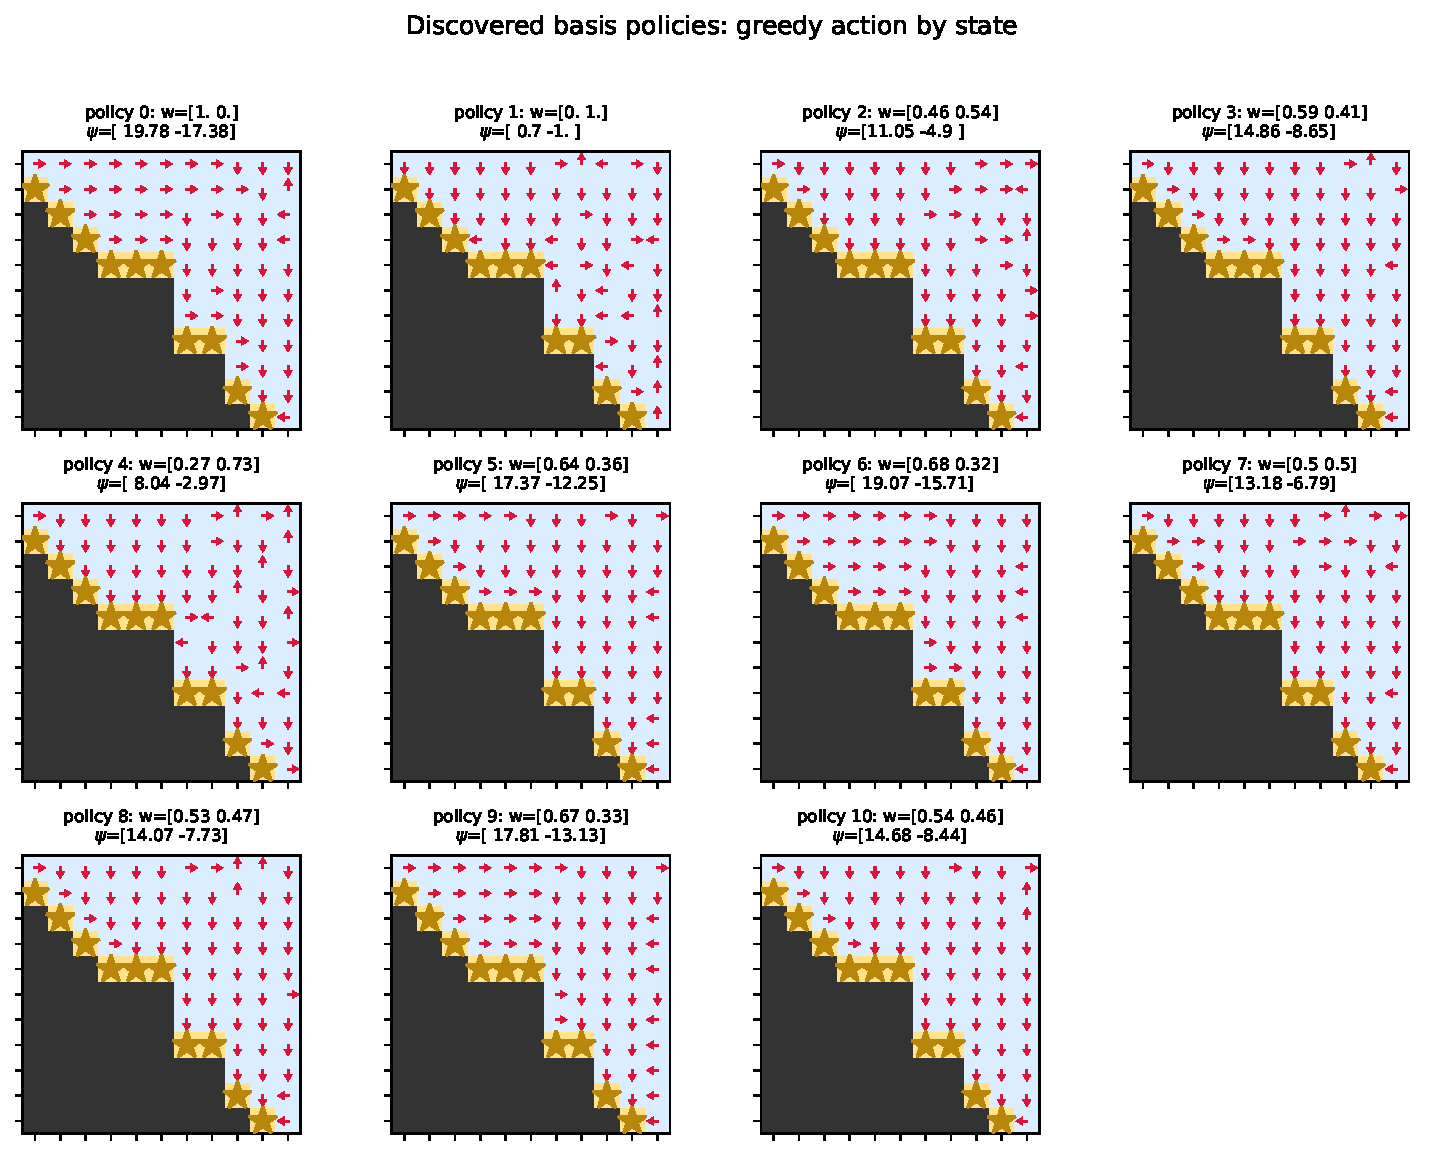
\includegraphics[width=\textwidth]{dst_02_4f616592}
\end{center}


For a random weight $\mathbf{w} = [0.2, 0.8]$ we reach optimality: 

\begin{center}
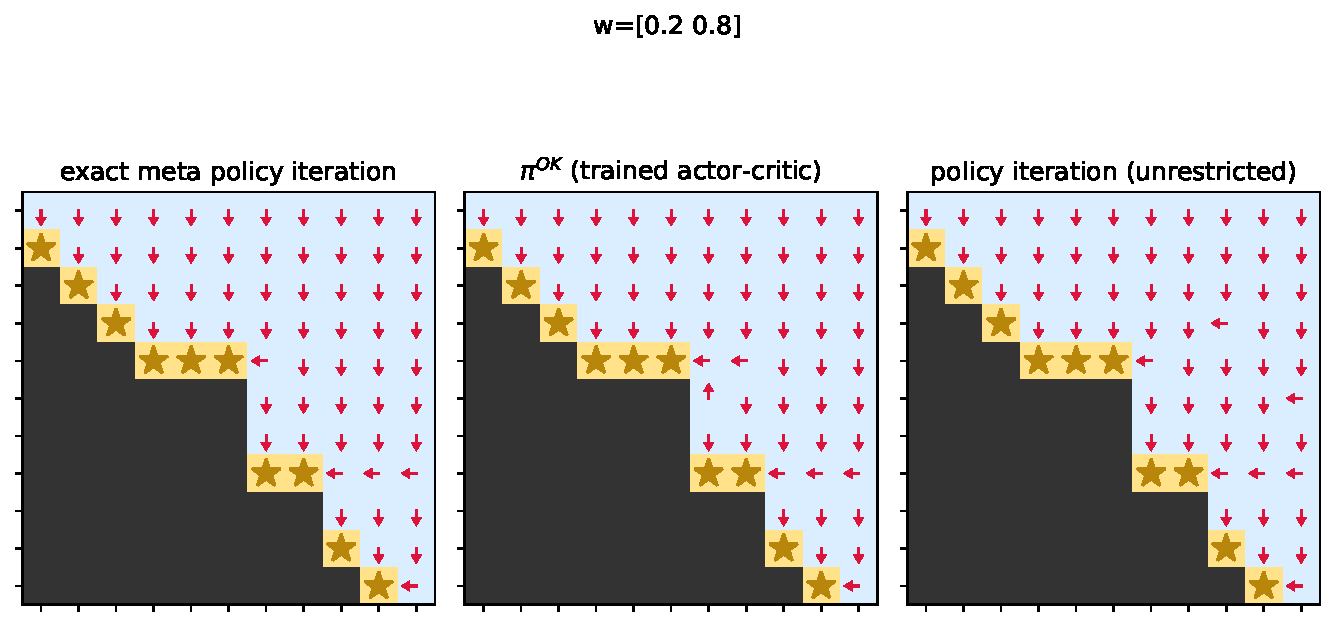
\includegraphics[width=0.85\textwidth]{dst_07_433edf00d77a}
\end{center}


\paragraph{Warm start:}\label{par:warmstart} Most of the times an optimal policy differs very slightly from the one obtained by GPI:
\[
\pi^{GPI}(s) = \argmax_{\pi \in \Pi} \psi^\pi(s,a) \cdot \mathbf{w} 
\] 

This motivates to start the Q-learning algorithm from $\pi^{GPI}$ via: 
\[
 q_w(s,a) = \max_j \psi^\pi_j \cdot \mathbf{w}
\]


\begin{center}
\begin{tabular}{lcc}
\toprule
 & median steps & median wall time \\
\midrule
standard & 12{,}500 & 1.241\,s \\
warm start (GPI init) & 1{,}500 & 0.144\,s \\
\bottomrule
\end{tabular}
\end{center}
Speedup $\mathbf{8.33}\times$ (steps) and $\mathbf{8.61} \times$ (wall time) taking median of 5 seeds each.

\paragraph{The metapolicy itself, learned online (\texttt{SFOLS/09\_qlearning\_metapolicy.ipynb}).} Every result
above solves the restricted operator $T_B$ exactly (dense linear algebra). Real SFOLS/GPI implementations
(\texttt{RM/sf-fsa-vi/sfols/rl/successor\_features/tabular\_sf.py}) learn $\Psi$ online via TD instead. We
re-implement Definition~\ref{def:meta}'s restricted composition with the identical SFQL-style TD update, restricting
both the $\varepsilon$-greedy behavior policy and the bootstrap target to $B(s)$, and compare it on DST against an
unrestricted learner trained from scratch for the same query weight, same schedule, same seeds:

\begin{center}
\begin{tabular}{lccc}
\toprule
 & 250 steps & 1000 steps & steps to converge \\
\midrule
restricted metapolicy & gap $=0.000$ & gap $=0.000$ & $\mathbf{250}$ \\
unrestricted, from scratch & gap $=1.706$ & gap $=0.000$ & $1000$ \\
\bottomrule
\end{tabular}
\end{center}
$\mathbf{4\times}$ fewer environment steps per query (mean of 10 seeds; gap to the exact optimum, DST, $w=(0.4,0.6)$),
after the $k=2$ base pool is built once ($16{,}000$ steps, amortized exactly as in every other speedup reported here).
Confirms Certify-or-Grow's restriction helps in the setting practitioners actually use, not only under exact solves.

\section{FSA (non-Markovian) on Policy basis}

We can grow the CCS and then perform the FSA-RM-VI algorithm. Or grow only the CCS to the size necessary to solve the FSA-RM-VI algorithm. The latter is the one we are going to present here.
\\


Let $v=\tau(u,\mathcal{O}(\varepsilon_j))$ and write $\widehat{W}[v] = W[v]/\|W[v]\|_1$ for
the normalized weight, assuming $W[v]\neq\mathbf{0}$. Then following Infante

\begin{align}
W^{k+1}[u]_j
&= \max_{a,\;\pi\in\Pi_{\mathrm{CCS}}}\ \psi^{\pi}(\varepsilon_j,a)^{\top}W^{k}[v]
\label{eq:infante11}\\[4pt]
&= \big\|W^{k}[v]\big\|_1 \cdot
   \max_{a,\;\pi\in\Pi_{\mathrm{CCS}}}\ \psi^{\pi}(\varepsilon_j,a)^{\top}\widehat{W}^{k}[v]
\label{eq:homog}\\[4pt]
&= \big\|W^{k}[v]\big\|_1 \cdot V^{*}_{\widehat{W}^{k}[v]}(\varepsilon_j)
\label{eq:gpi}\\[4pt]
&= \big\|W^{k}[v]\big\|_1 \cdot \Psi^{\pi_{\mathrm{meta}}}(\varepsilon_j,\pi_{\mathrm{meta}}(\varepsilon_j))^\top\widehat W^{k}[v],
\label{eq:cog}\\[4pt]
&\hspace{2cm}(\pi_{\mathrm{meta}},\Psi^{\pi_{\mathrm{meta}}},\mathcal{B}) \gets \textsc{Certify-or-Grow}\big(\widehat{W}^{k}[v],\,\mathcal{B}\big).\notag
\end{align}


\begin{algorithm}[H]
\caption{\textsc{Certified-RM-VI}}
\begin{algorithmic}[1]
\State $\mathcal{B}\gets\emptyset$;\quad $\mathcal P\gets\emptyset$ \Comment{pool of solved metapolicies, GPI-ready}
\State $W[u]\gets\mathbf{0}\in\mathbb{R}^{|E|}$ for all $u\in U$
\Repeat
  \For{each $u$, each distinct successor $v$ of $u$}
    \State $E_{uv}\gets\{\,j:\tau(u,\mathcal{O}(\varepsilon_j))=v\,\}$
    \If{$v$ terminal}
      \State $W[u]_j\gets r(u,v)$ for $j\in E_{uv}$
    \Else
      \State $\pi_{\mathrm{meta}},\Psi^{\pi_{\mathrm{meta}}},\;\mathcal{B}\gets\textsc{Certify-or-Grow}\big(W[v]/\|W[v]\|_1,\;\mathcal{B}\big)$
      \State $\mathcal P\gets\mathcal P\cup\{(\pi_{\mathrm{meta}},\Psi^{\pi_{\mathrm{meta}}})\}$ \Comment{same fix as Remark~\ref{rem:pool-closes-gap}: cache the full table, not just the exit value}
      \State $W[u]_j\gets\|W[v]\|_1\cdot\Psi^{\pi_{\mathrm{meta}}}(\varepsilon_j,\pi_{\mathrm{meta}}(\varepsilon_j))^\top(W[v]/\|W[v]\|_1)$ for $j\in E_{uv}$
    \EndIf
  \EndFor
\Until{$\|W-W_{\mathrm{prev}}\|_\infty\le\varepsilon$}
\For{each $u$}
  \State $\pi_{\mathrm{meta}},\Psi^{\pi_{\mathrm{meta}}},\;\mathcal{B}\gets\textsc{Certify-or-Grow}\big(W[u]/\|W[u]\|_1,\;\mathcal{B}\big)$
  \State $\mathcal P\gets\mathcal P\cup\{(\pi_{\mathrm{meta}},\Psi^{\pi_{\mathrm{meta}}})\}$
\EndFor
\State \Return $W$, $\mathcal{B}$, $\mathcal P$
\end{algorithmic}
\end{algorithm}

\begin{remark}[Coverage gap]
The sweep only ever queries $W[v]$ at edge \emph{targets}. The start state is never certified during the loop, even though the acting policy at $u_0$ still needs $V^{\pi(W[u_0])}$ to be exact, we fix it in the post certification.
\end{remark}

\paragraph{Results (Office domain, ``coffee $\to$ mail $\to$ office'')}

\begin{center}
\begin{tabular}{lccc}
\toprule
 & basis size & sweeps & median time \\
\midrule
standard (SFOLS discovers CCS, then traverse) & 17 exact solves & 4 & 40886.4\,ms \\
certified/adaptive, exact (ours) & 3 exact solves (3 distinct) & 4 & 2997.9\,ms \\
\bottomrule
\end{tabular}
\end{center}

The speed up in this algorithm is of about $\textbf{13.64} \times$.

\begin{remark}[Domain-specific basis size]
Office's domain only needs the $d=6$ canonical corners to perform Infante's algorithm succesfully. Our adaptative basis reduces this to $3$ distinct corners, however it will need to compute other policies if the higher MDP is rewriten.
\end{remark}


\paragraph{To do:}

\begin{itemize}
    \item Backpropagation of Certified-RM-VI can be optimized. 
    \item What happens with continous MORL? 
    \item What happens with other high-level tasks.
\end{itemize}


\subsection{Exact one-step adjacency characterizes the $k=1$ gap}

\begin{proposition}[Single-policy case]\label{prop:adjacency}
Single-pickup-terminal MO-MDP with reward states $R_1,\dots,R_d$ ($\phi(s,a)=e_i$ iff $a$ leads directly to $R_i$,
terminal on arrival, $0$ otherwise). Let $\mathcal B=\{\pi_1\}$, $\pi_1$ exactly optimal for $e_1$. If no state on
$\pi_1$'s trajectory from $s$ is one step from $R_j$ for any $j\ne1$, then
$\pi^{\mathrm{GPI}}_{\mathcal B}(s;w)=\pi_{\mathrm{meta}}(s;w)=\pi_1(s)$ for every $w$ with $w_1>0$.
\end{proposition}

\begin{proof}
$B(s)=\{\pi_1(s)\}$, so $\pi_{\mathrm{meta}}(s)=\pi_1(s)$ trivially. For GPI: $\pi_1$'s own continuation from any
state never visits another reward (same hypothesis, applied recursively), so
$\Psi^{\pi_1}(s',\pi_1(s'))=c(s')e_1$ for some $c(s')\ge0$. No action from $s$ reaches $R_j$, $j\ne1$, in one step,
so $\phi(s,a)^\top w\in\{0,w_1\}$ for every $a$, giving
$\Psi^{\pi_1}(s,a)^\top w = w_1\cdot\big[\mathbb 1(a\text{ reaches }R_1)+\gamma c(s'(a))\,\mathbb 1(\text{else})\big]
= w_1\cdot\Psi^{\pi_1}(s,a)^\top e_1$,
a positive ($w_1>0$) rescaling of $\Psi^{\pi_1}(s,a)^\top e_1$, hence maximized at the same $a=\pi_1(s)$ that
maximizes the latter, by definition of $\pi_1$'s own optimality.
\end{proof}

Confirmed by direct sweep (\texttt{SFOLS/07\_proximity\_sweep.ipynb}):
$\pi^{\mathrm{GPI}}_{\mathcal B}=\pi_{\mathrm{meta}}$ exactly for every tested adjacency distance $d\ge2$, with a
strict, nonzero gap appearing only at $d=1$.

\paragraph{Measured cost of iterating $\pi^{\mathrm{hyb}}$ to full optimality (Office, canonical-corner basis
$k=1,\dots,6$, 30 test weights).} Each $k$ warm-starts the same full-action-set policy-iteration loop at
$\pi_{\mathrm{meta}}$'s own greedy policy and counts sweeps to the fixed point, against a cold start
(\texttt{policy}$=0$ everywhere, Line~\ref*{alg:cog-fallback}'s current behavior):

\begin{center}
\begin{tabular}{lccc}
\toprule
 & mean sweeps & min / max sweeps & speedup vs.\ cold \\
\midrule
cold start (current fallback) & 16.13 & 10 / 21 & --- \\
$k=1$ & 14.10 & 2 / 24 & $1.14\times$ \\
$k=2$ & 12.87 & 2 / 24 & $1.25\times$ \\
$k=3$ & 12.07 & 2 / 24 & $1.34\times$ \\
$k=4$ & 9.93  & 2 / 24 & $1.62\times$ \\
$k=5$ & 7.03  & 2 / 24 & $2.29\times$ \\
$k=6$ & 3.83  & 2 / 10 & $\mathbf{4.21\times}$ \\
\bottomrule
\end{tabular}
\end{center}

Mean cost drops monotonically as the basis grows: a $4.21\times$ reduction in exact-solve sweeps at the complete
basis, consistent in kind with the $8.33\times$ Q-learning warm-start speedup reported above
(p.\pageref{par:warmstart}). Two caveats keep this honest rather than optimistic:

\begin{remark}[The ``already stable'' certificate never fired, even at $k=6$]
Not one of the 30 weights reached $\pi^{\mathrm{hyb}}=\pi_{\mathrm{meta}}$'s own action in a single sweep, even
though $k=6$'s basis makes $V_{\mathrm{meta}}=V^*_w$ exactly in this domain. Office's terminate-on-any-object
structure produces many tied $Q$-values, and $\arg\max$ breaks ties by lowest index — so the freshly-recomputed
full-action greedy action can differ in \emph{label} from $\pi_{\mathrm{meta}}$'s own choice while being equal in
\emph{value}, costing one wasted-but-value-neutral extra sweep. The real certificate is the Bellman-gap test (as
in \texttt{meta\_policy\_iteration\_certified}), not exact policy equality — the gap is zero at $k=6$ even though
the sweep count never bottoms out at exactly $1$.
\end{remark}

\begin{remark}[Worst-case sweeps are not monotone in $k$]
The maximum over the 30 weights stays at $24$ — worse than the cold start's own worst case of $21$ — for every
$k \le 5$, dropping to $10$ only at $k=6$. A value estimate numerically close to $V^*_w$ does not guarantee its
greedy policy is close in \emph{policy space}: tie-heavy domains like Office can thrash between equally-good
actions for several rounds before settling. So the warm start is a better bet \emph{on average}, not a
per-instance guarantee.
\end{remark}

\pagebreak

\section{DST}

\begin{center}
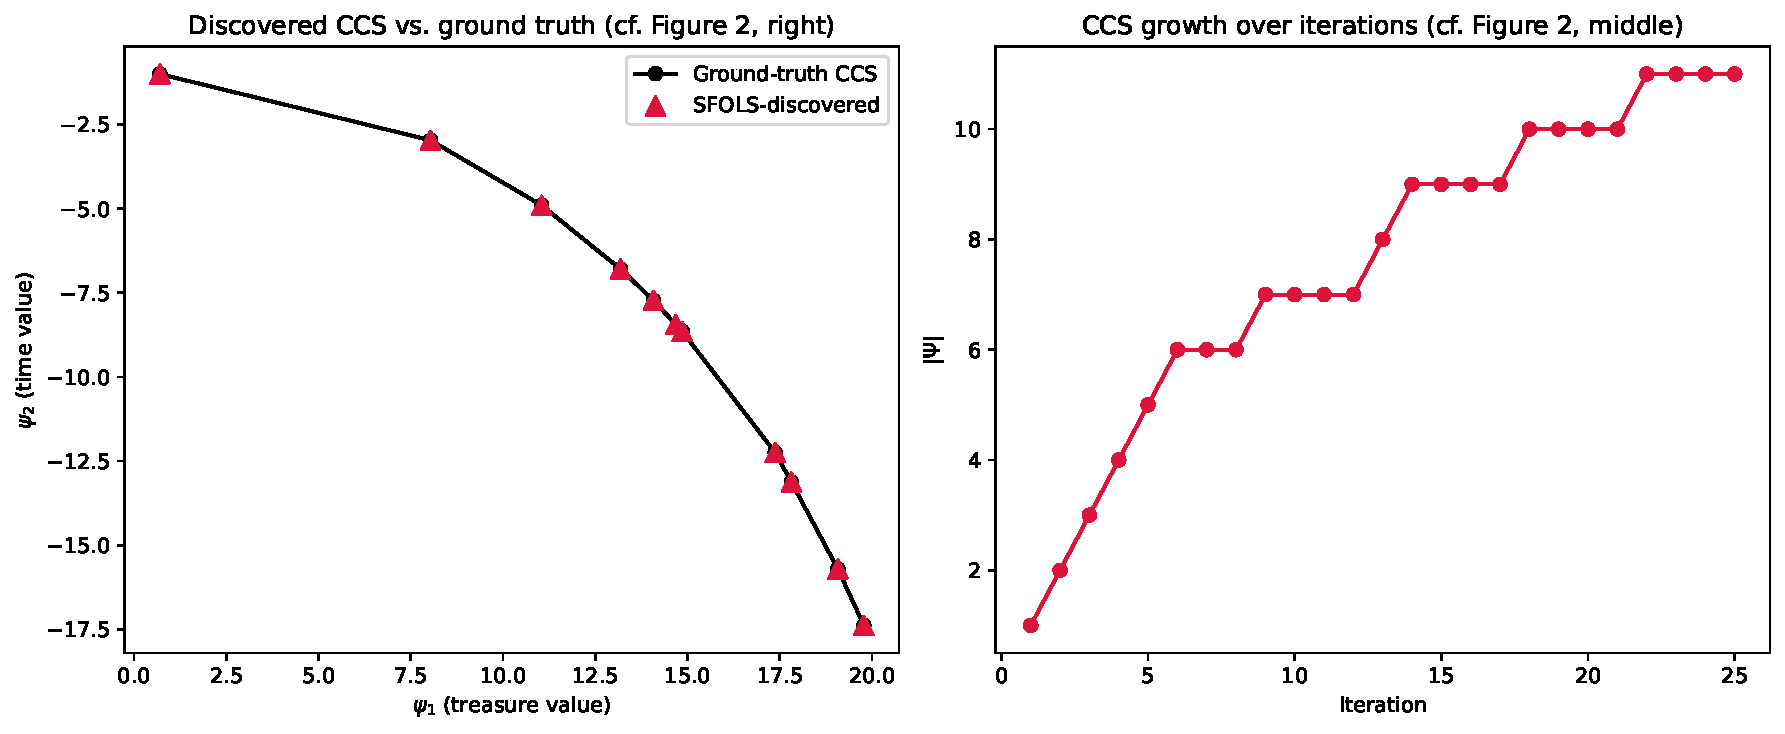
\includegraphics[width=0.85\textwidth]{dst_01_a0db2500}
\end{center}
\begin{center}
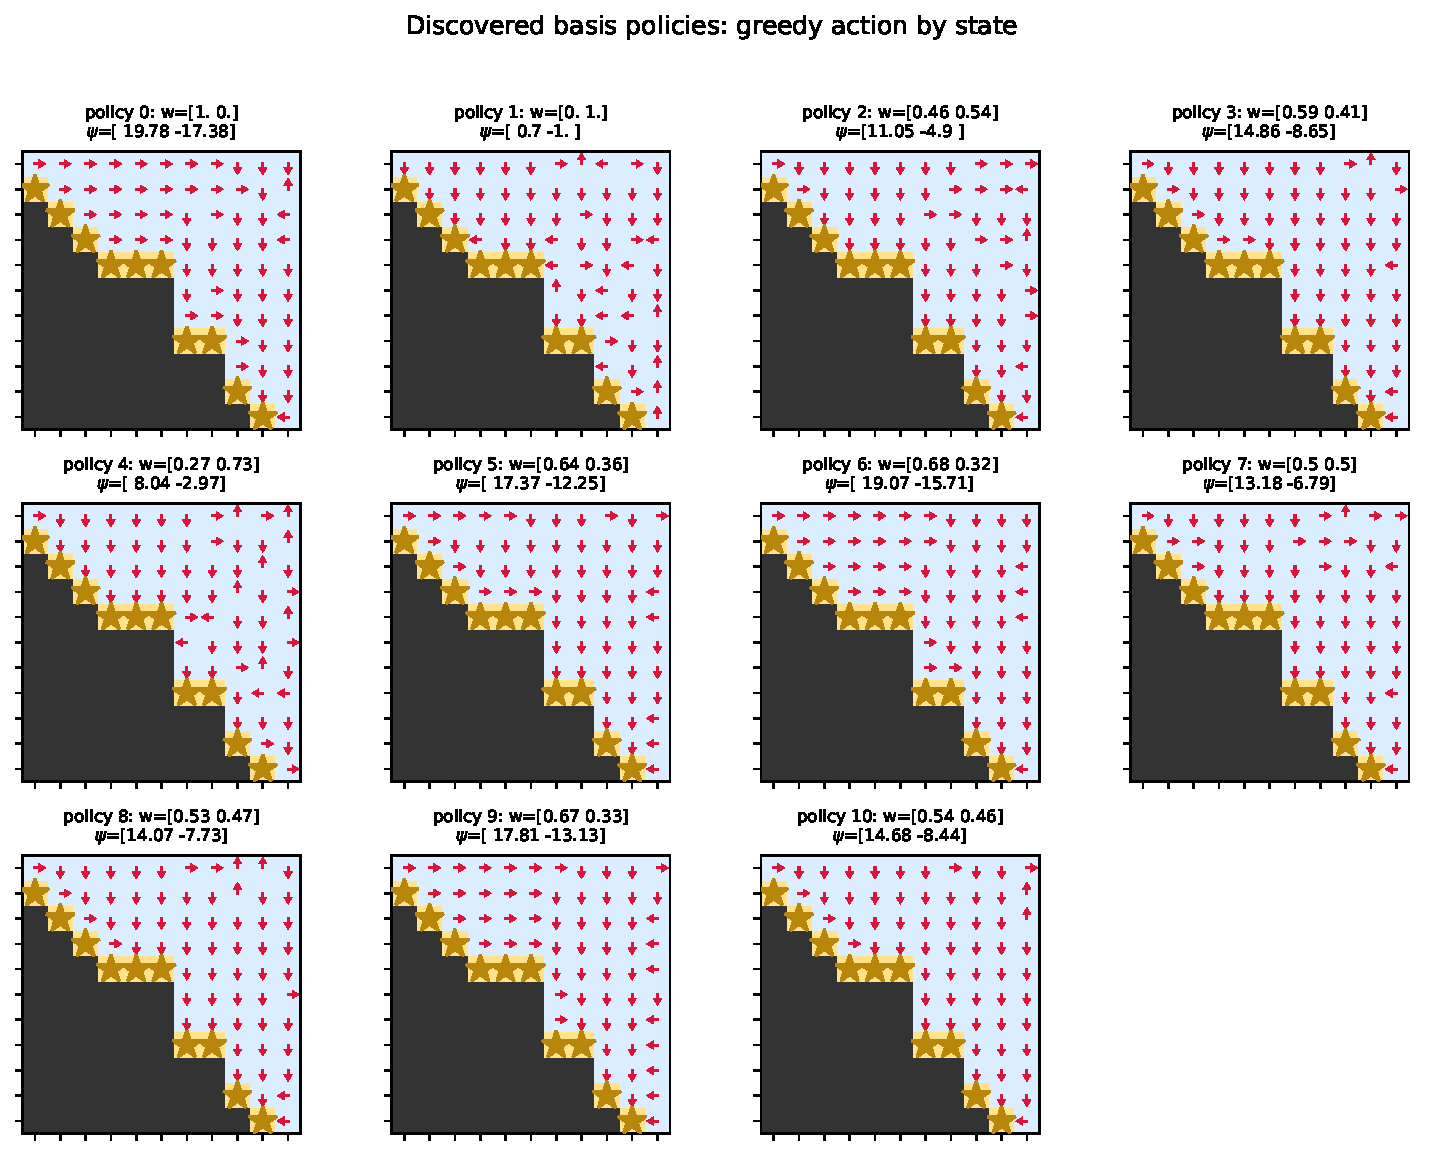
\includegraphics[width=0.85\textwidth]{dst_02_4f616592}
\end{center}
\begin{center}
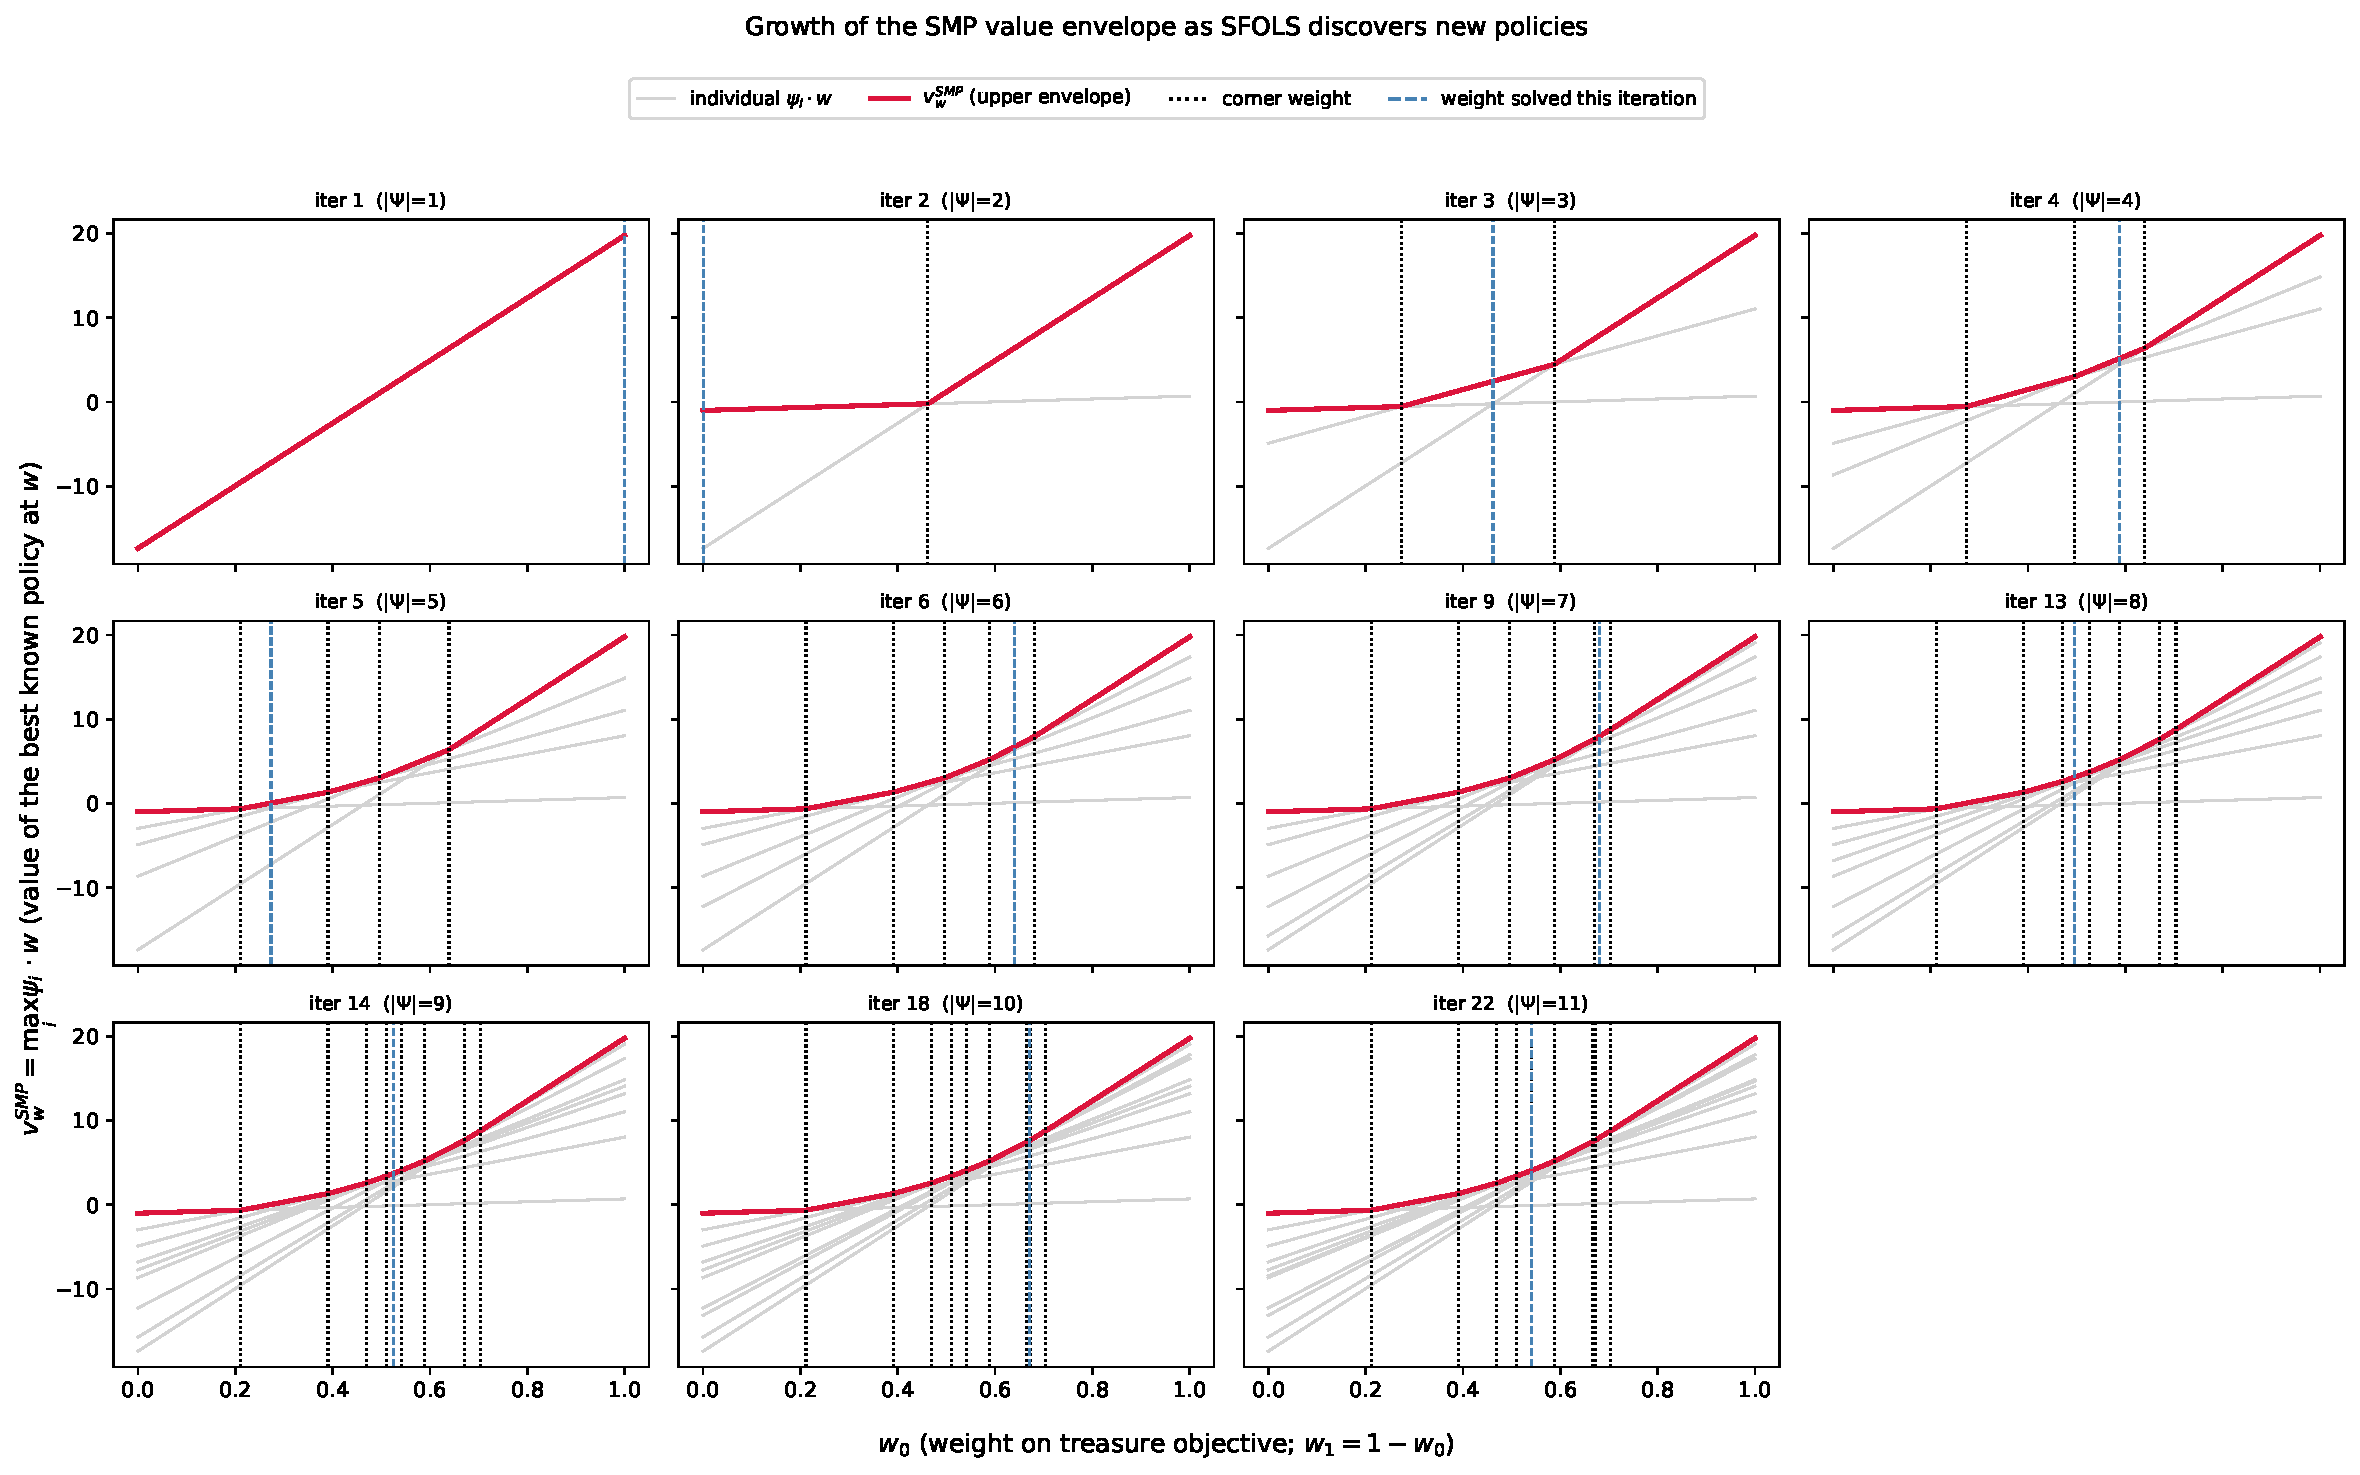
\includegraphics[width=0.85\textwidth]{dst_03_a849d4ab}
\end{center}
\begin{center}
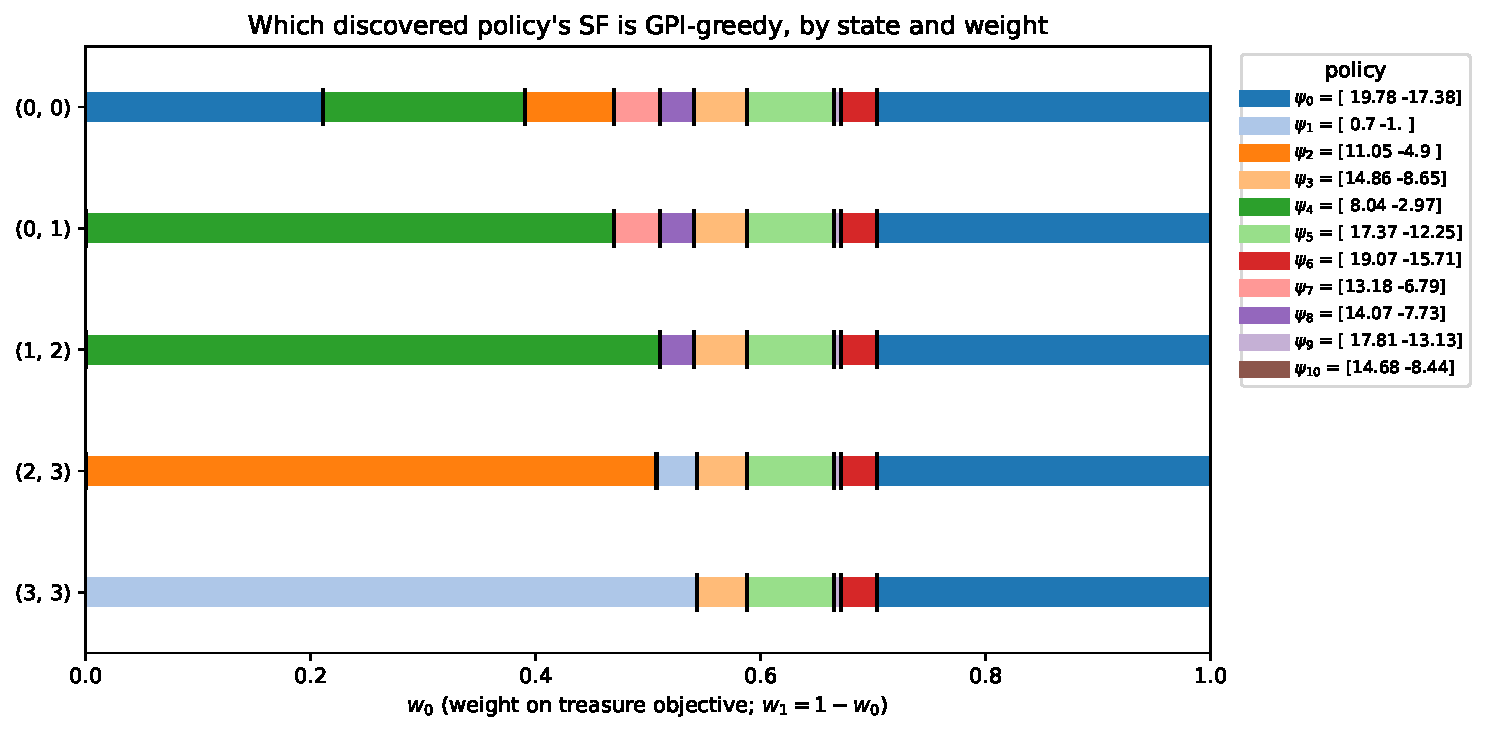
\includegraphics[width=0.85\textwidth]{dst_04_0f9545ec}
\end{center}
\begin{center}
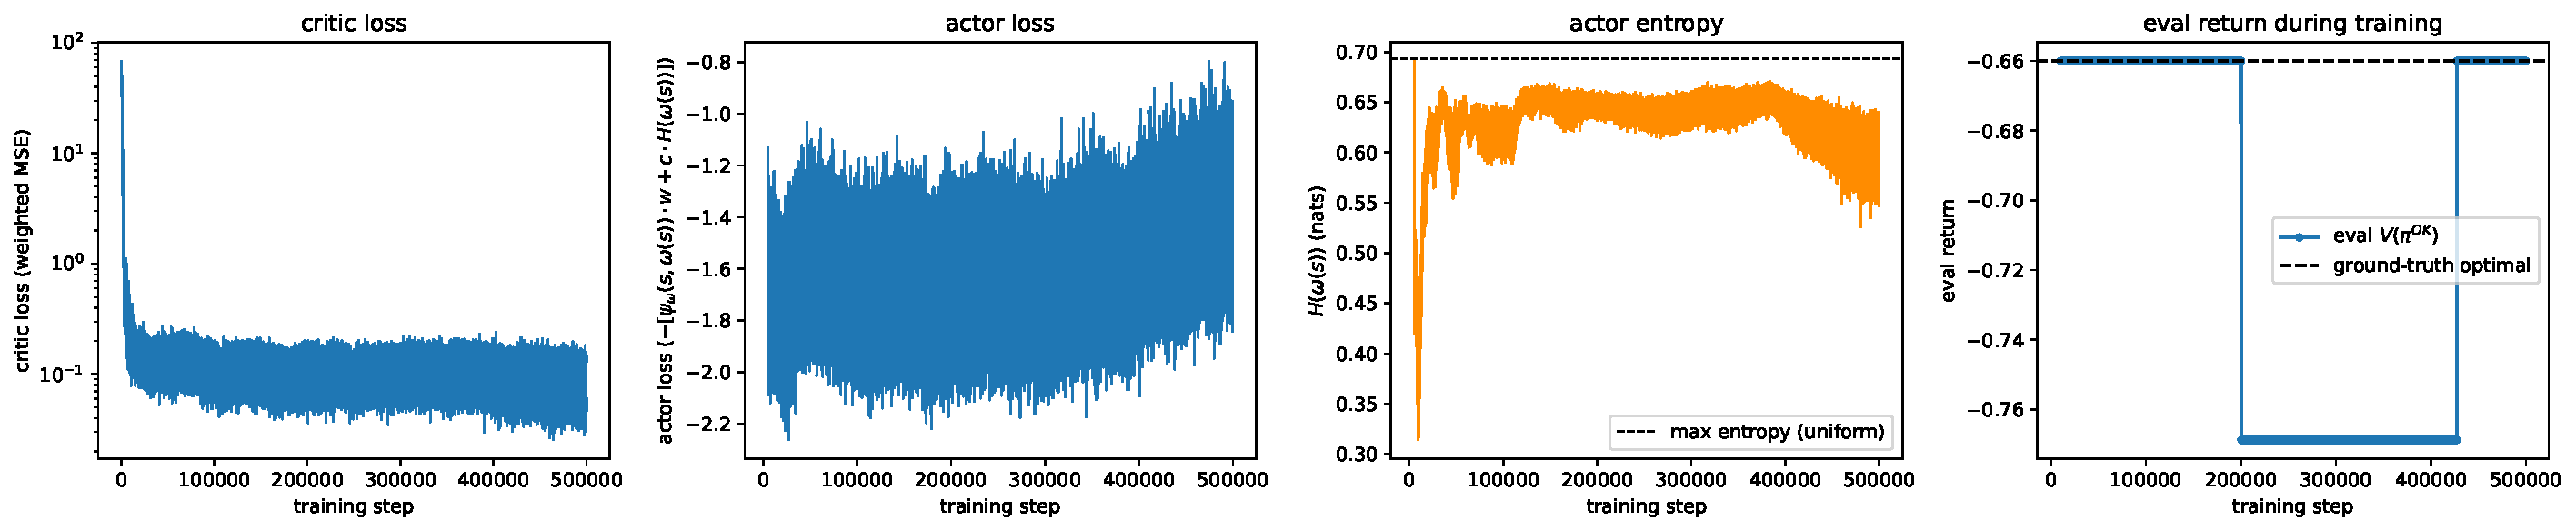
\includegraphics[width=0.85\textwidth]{dst_05_trainlosscurv}
\end{center}
\begin{center}
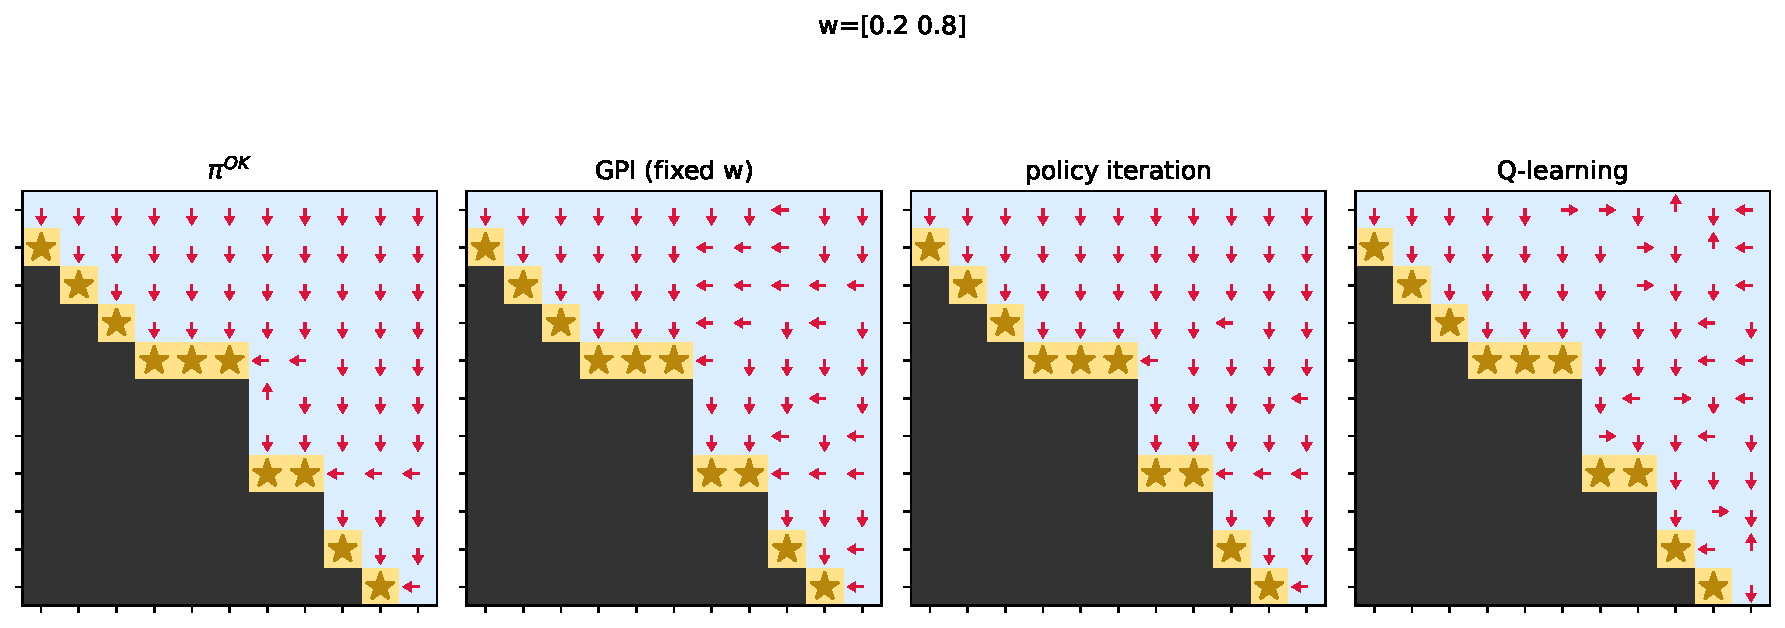
\includegraphics[width=0.85\textwidth]{dst_06_9e412238}
\end{center}
\begin{center}
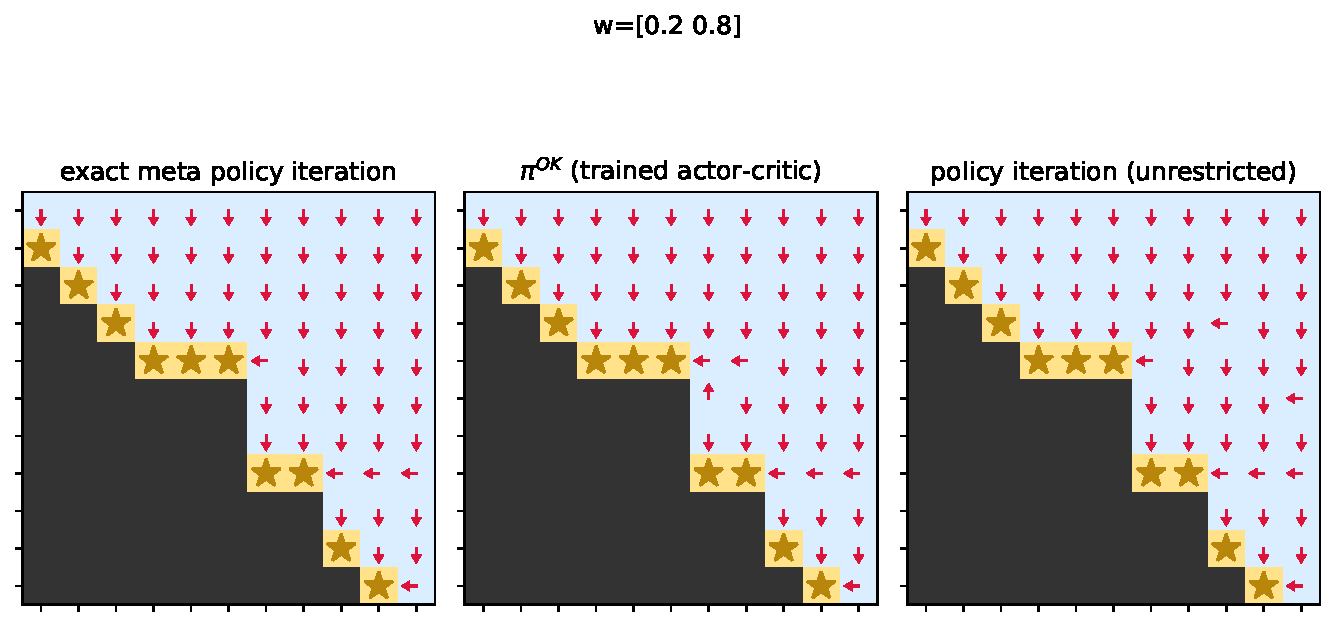
\includegraphics[width=0.85\textwidth]{dst_07_433edf00d77a}
\end{center}
\begin{center}
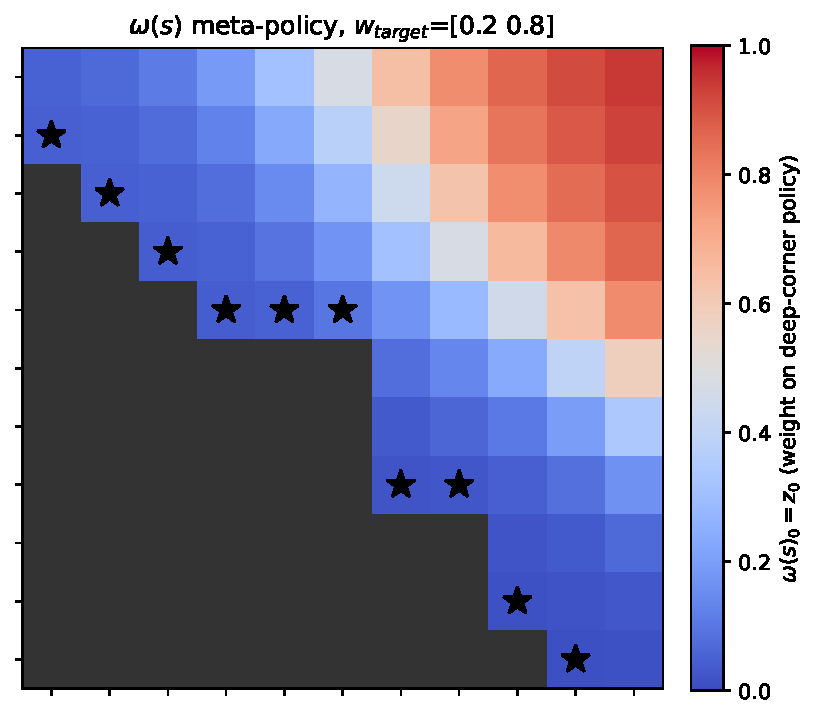
\includegraphics[width=0.6\textwidth]{dst_08_omegaheatmap0}
\end{center}
\begin{center}
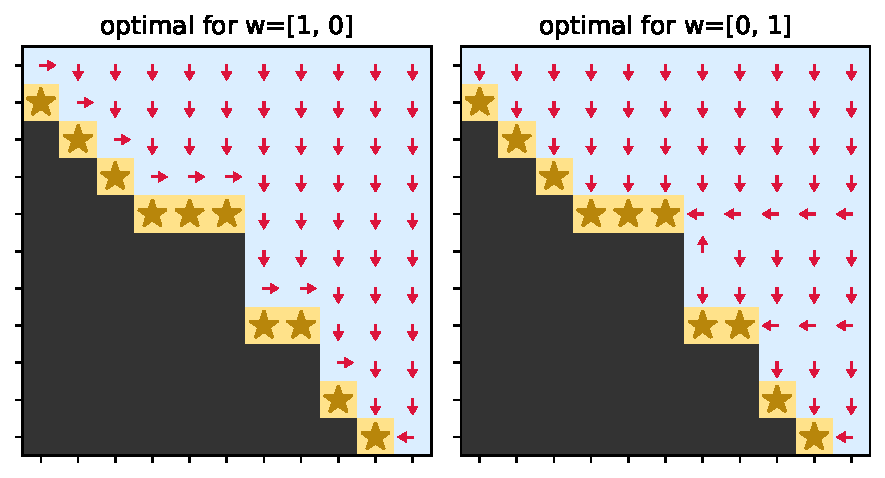
\includegraphics[width=0.6\textwidth]{dst_09_955e55b9}
\end{center}
\begin{center}
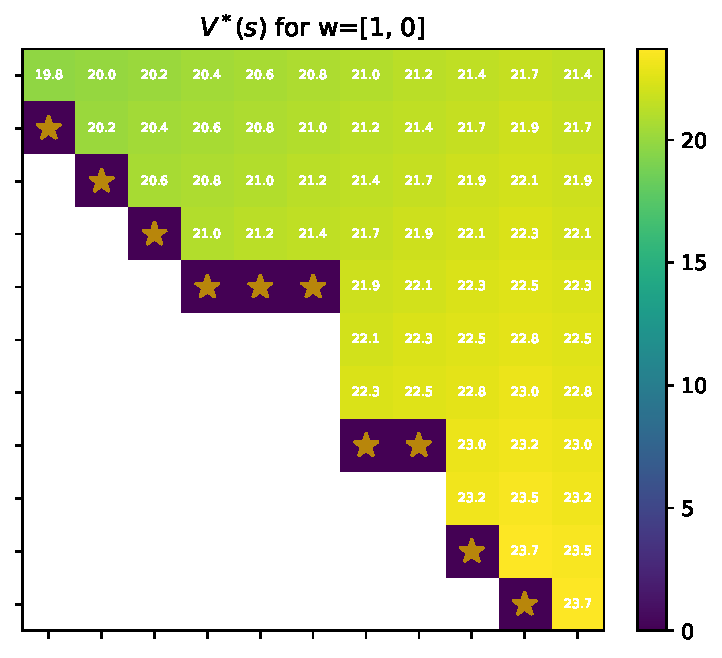
\includegraphics[width=0.6\textwidth]{dst_10_6c664da5}
\end{center}
\begin{center}
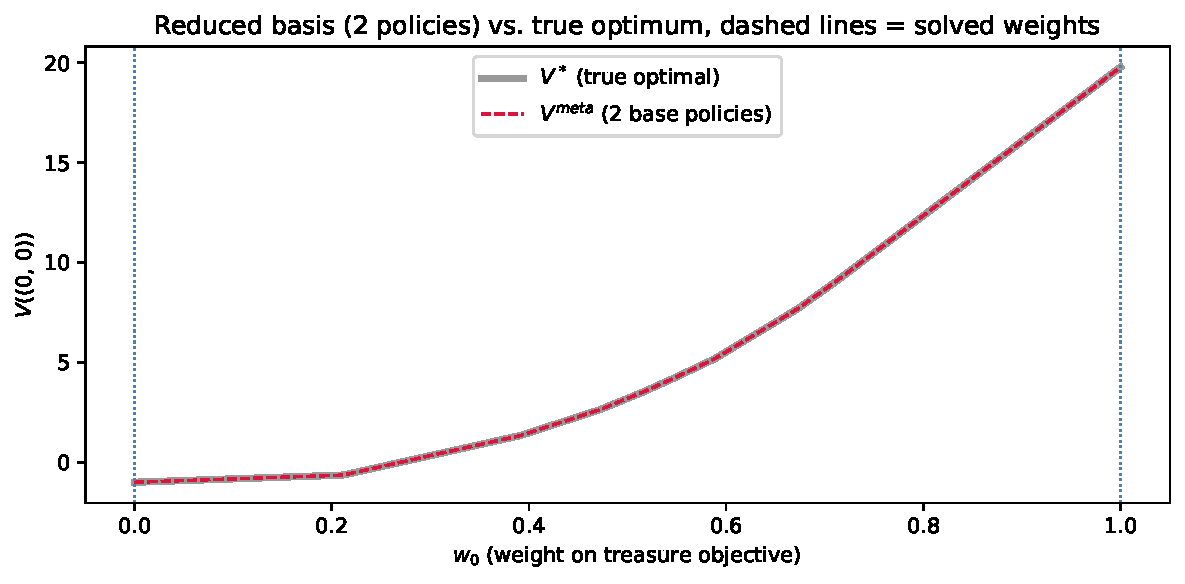
\includegraphics[width=0.7\textwidth]{dst_11_590e08cd88f5}
\end{center}

\section{Office}

\begin{center}
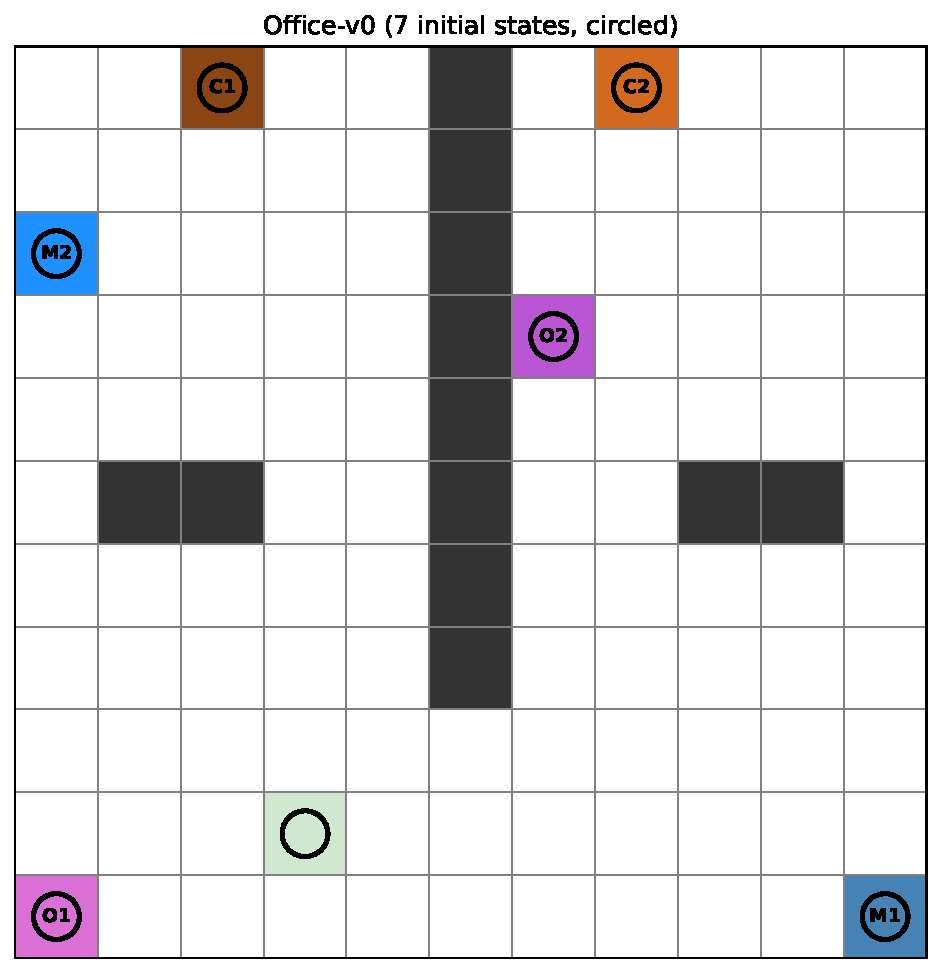
\includegraphics[width=0.6\textwidth]{office_01_domainmap}
\end{center}
\begin{center}
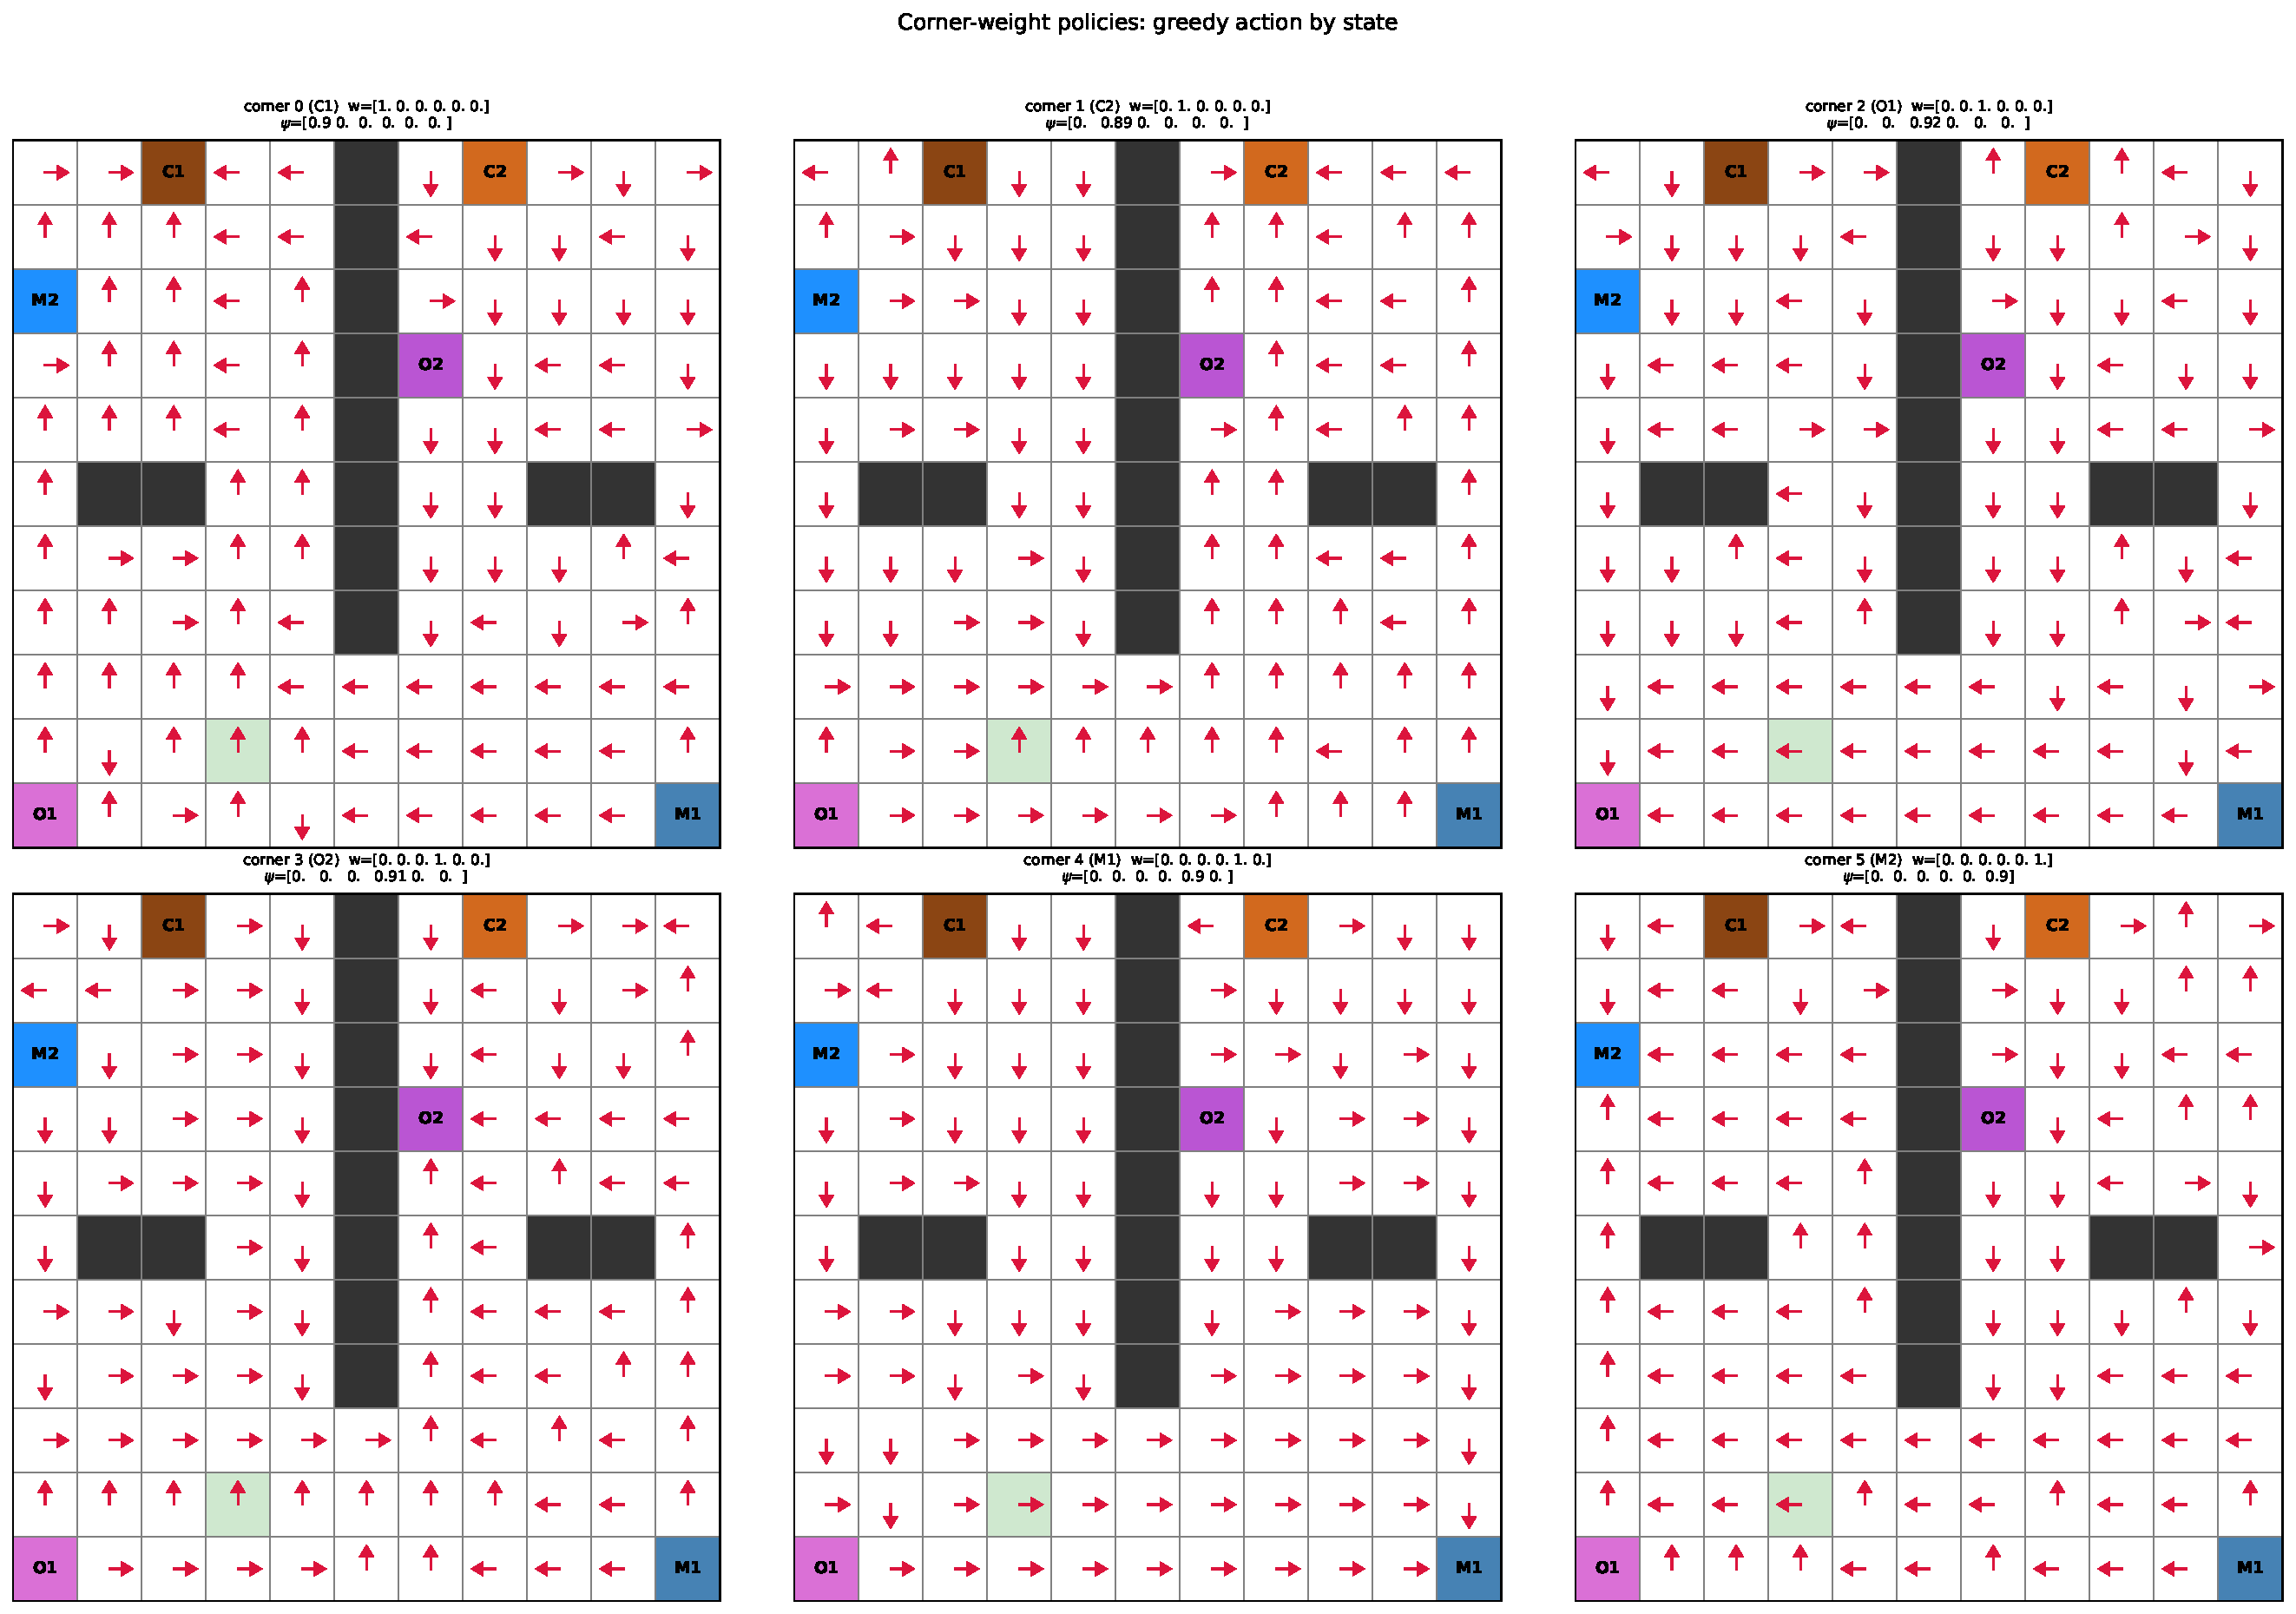
\includegraphics[width=0.85\textwidth]{office_02_cornerpolicies}
\end{center}
\begin{center}
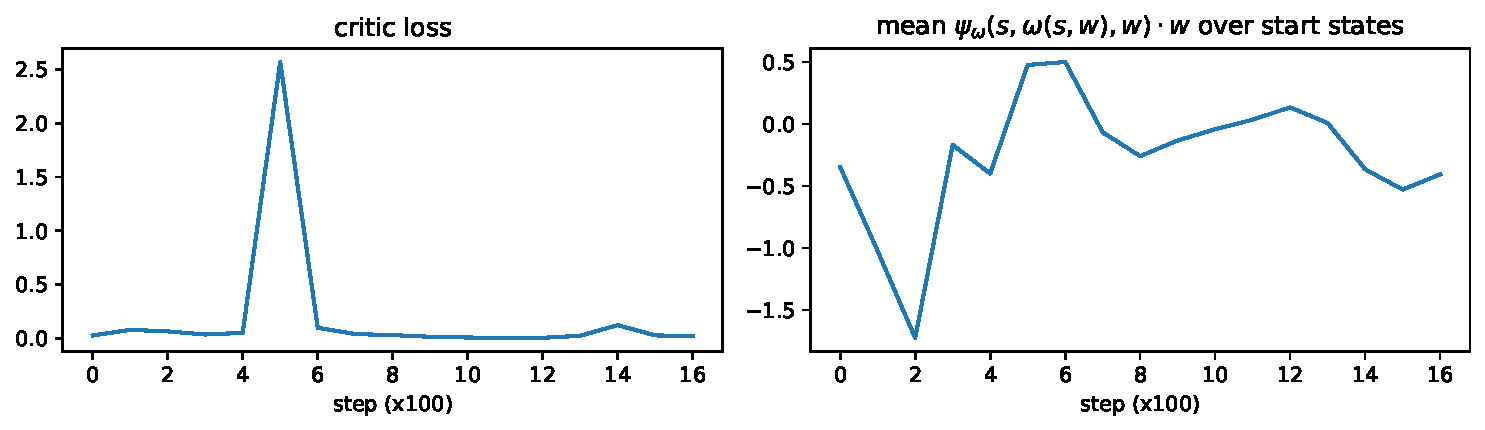
\includegraphics[width=0.85\textwidth]{office_03_trainlosscurv}
\end{center}
\begin{center}
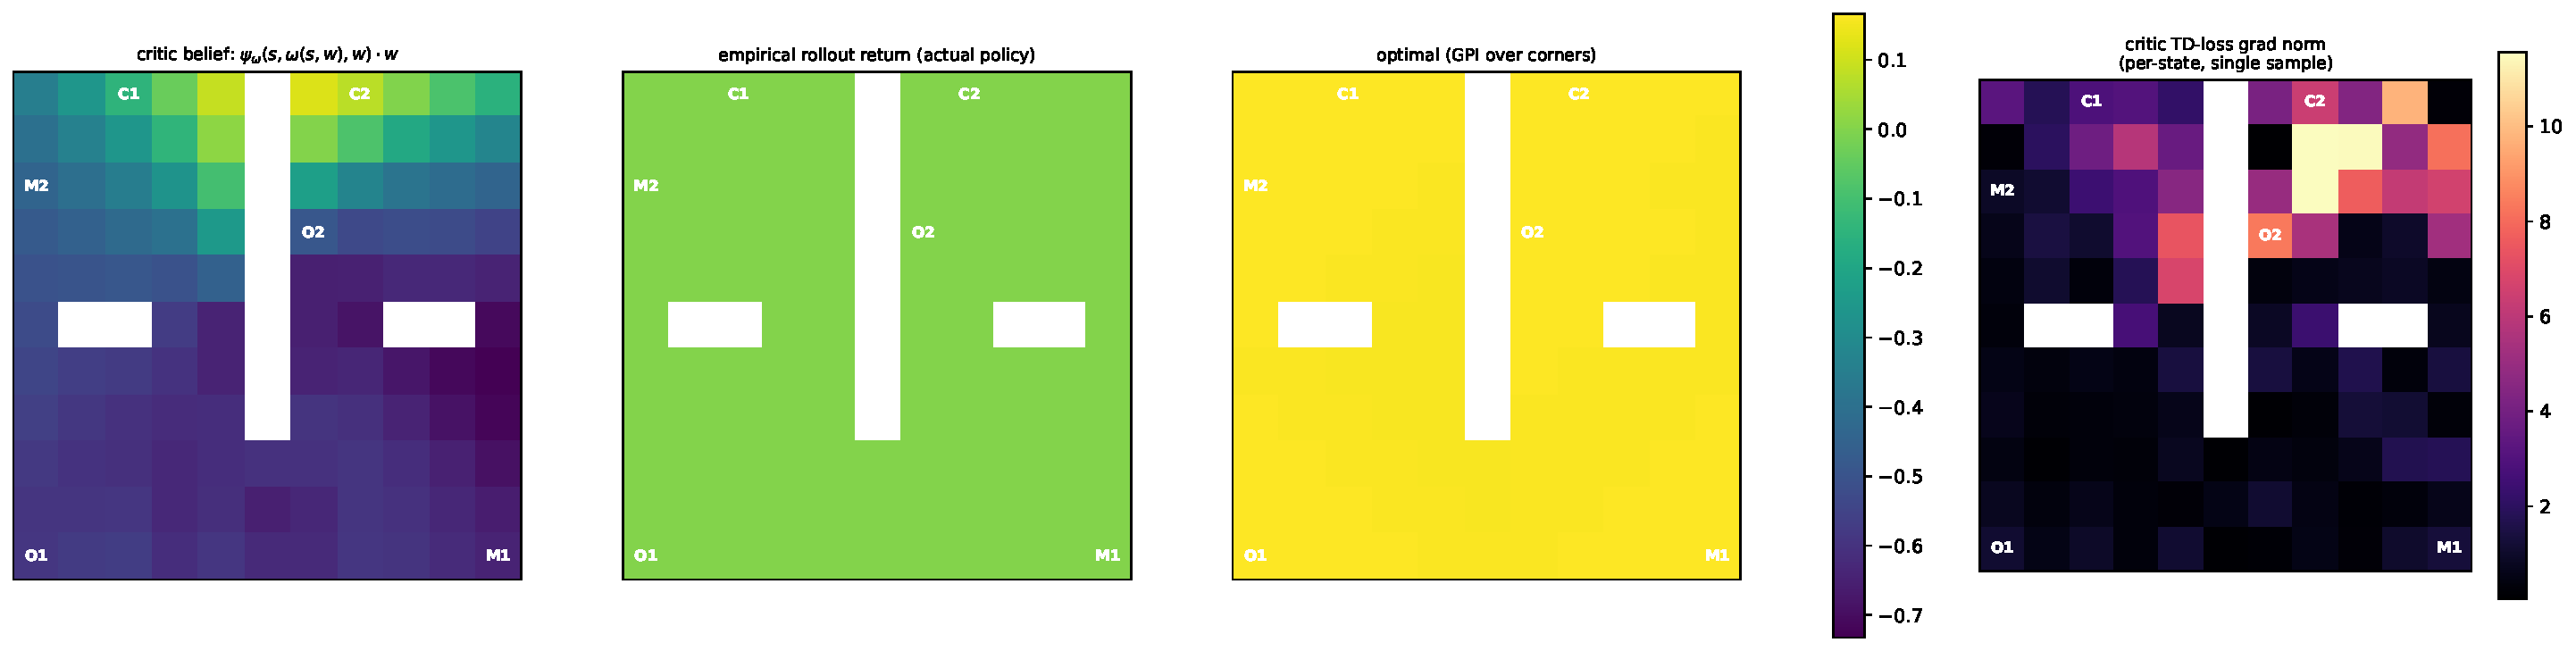
\includegraphics[width=0.85\textwidth]{office_04_valuemaps}
\end{center}
\begin{center}
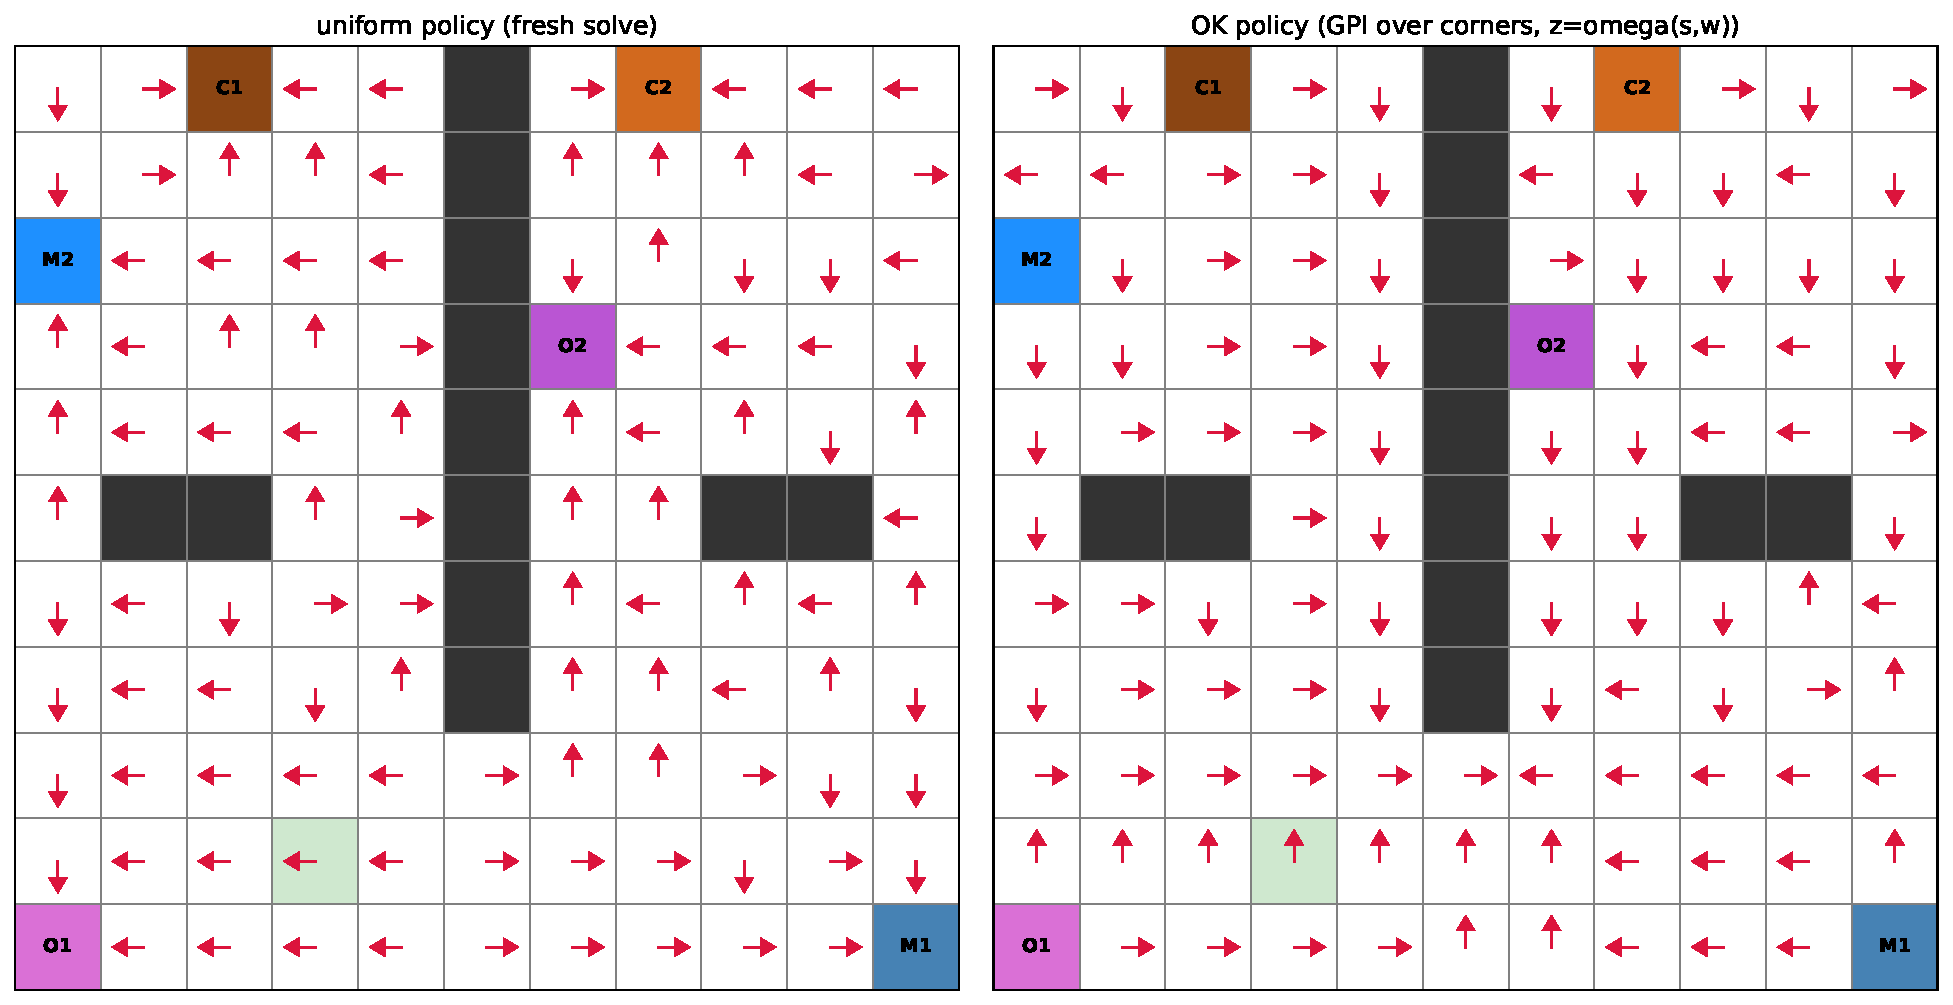
\includegraphics[width=0.85\textwidth]{office_05_uniformvsok}
\end{center}
\begin{center}
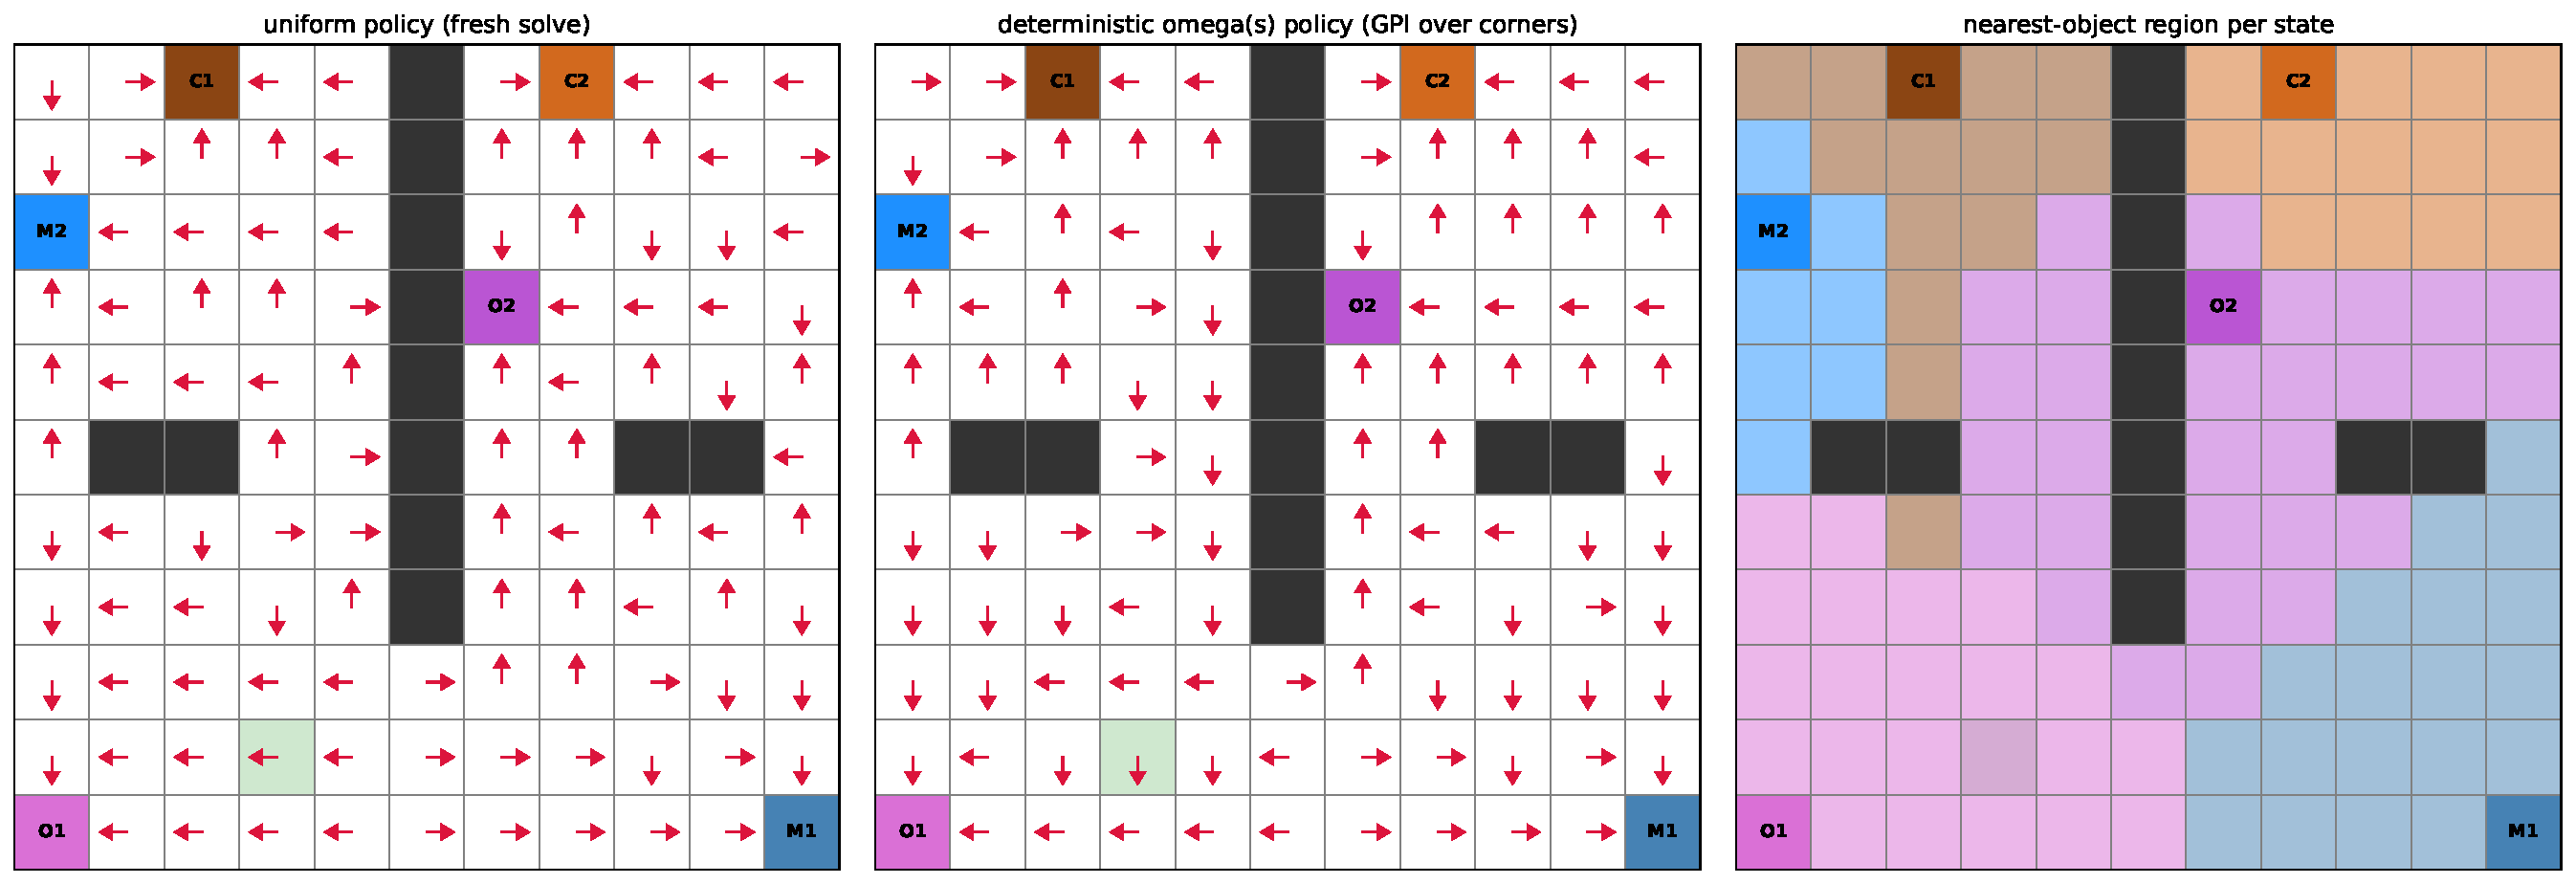
\includegraphics[width=0.85\textwidth]{office_06_uniformvsdetomega}
\end{center}
\begin{center}
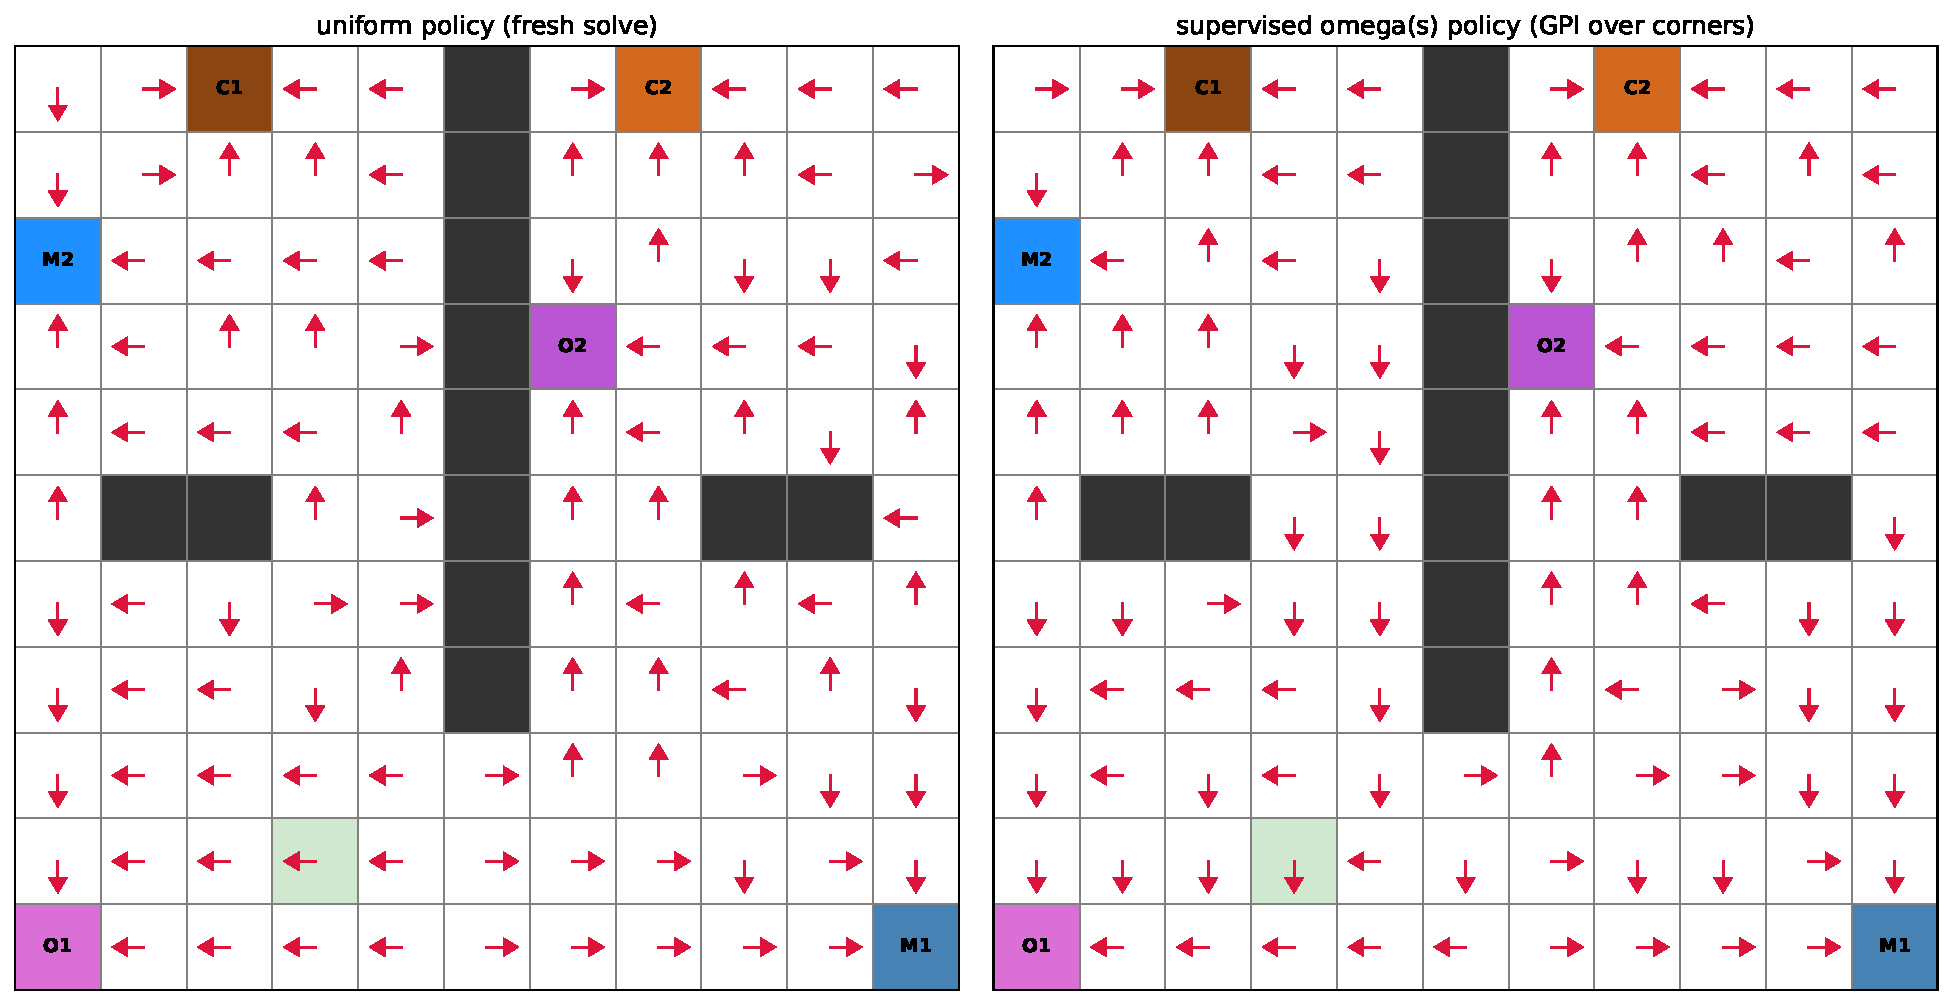
\includegraphics[width=0.85\textwidth]{office_07_uniformvssupervised}
\end{center}
\begin{center}
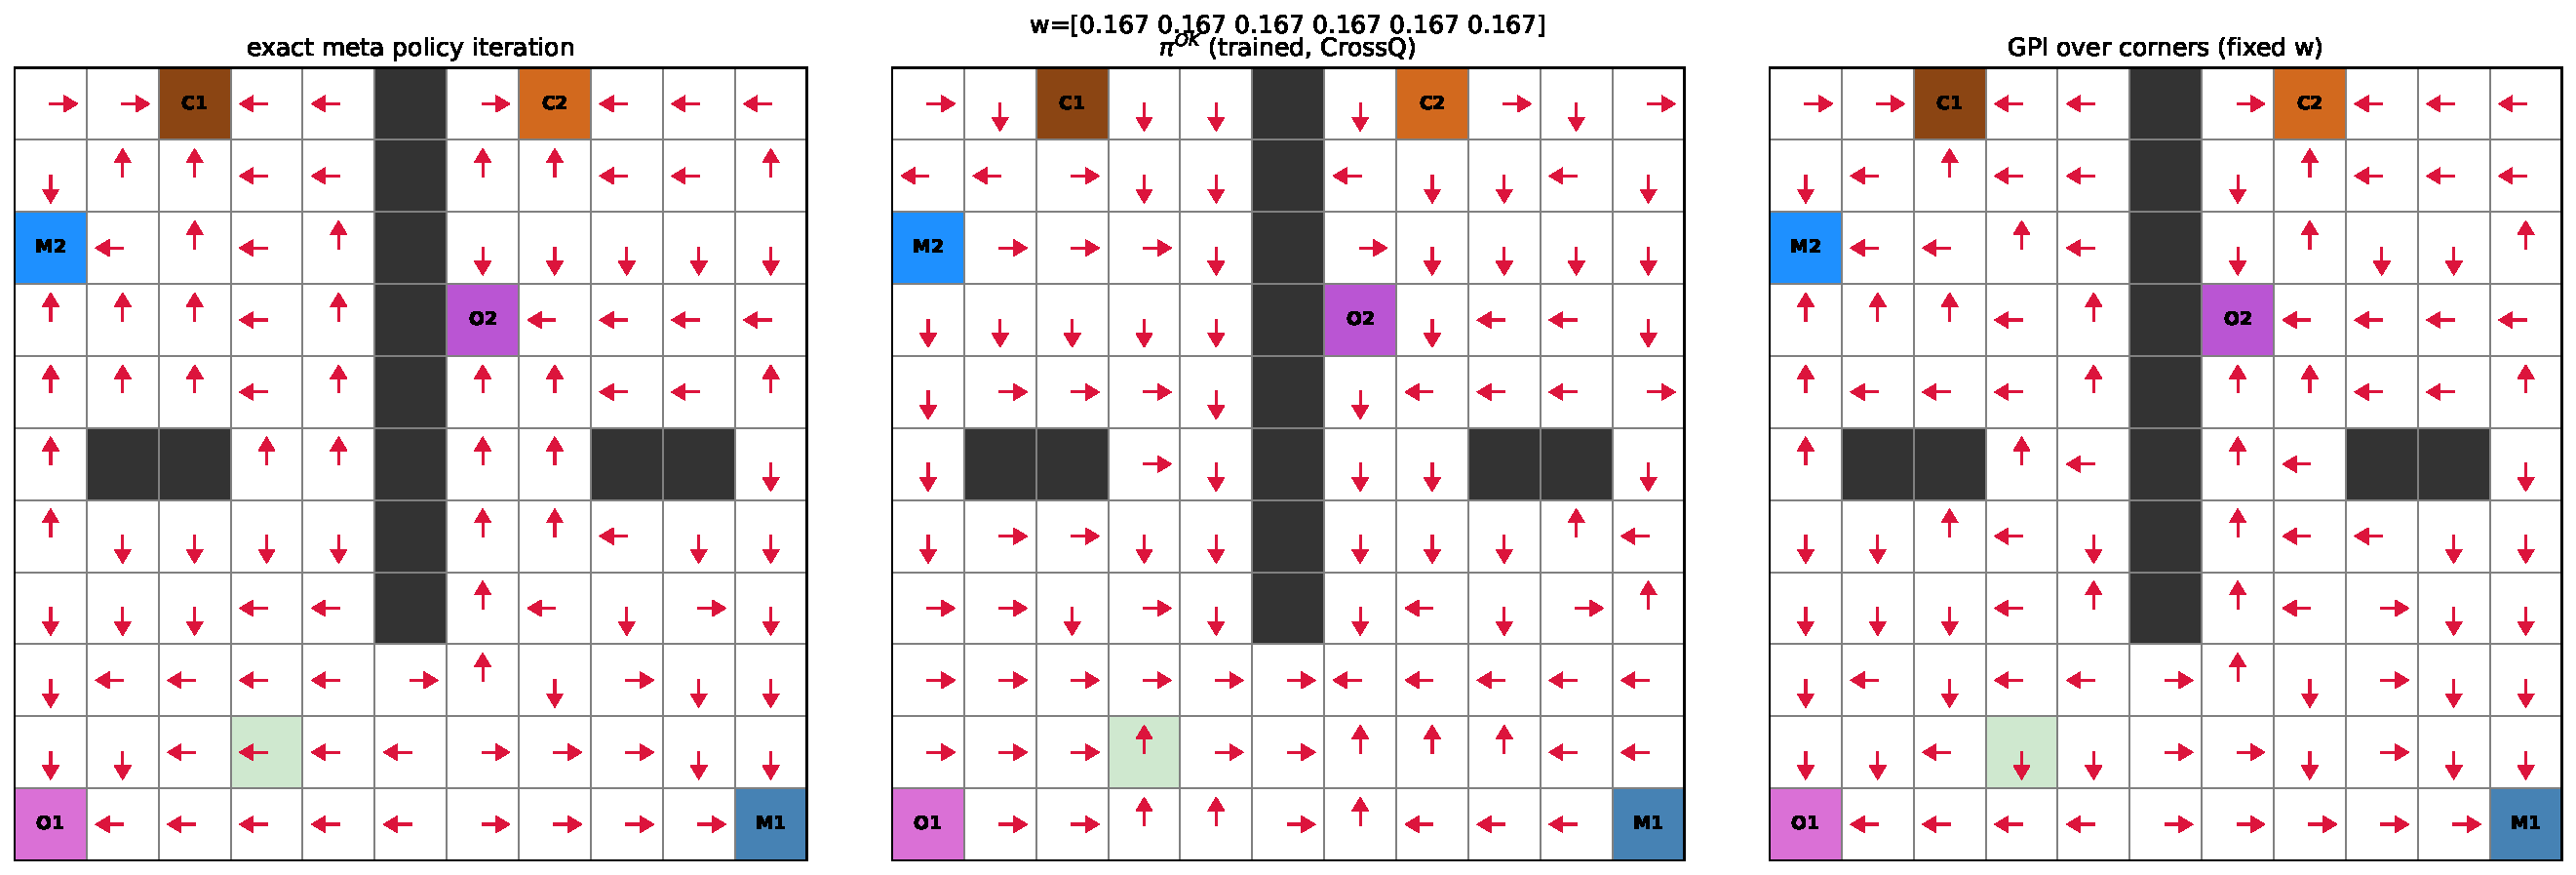
\includegraphics[width=0.85\textwidth]{office_08_metavsokvsgpi}
\label{fig:office-metavsokvsgpi}
\end{center}
\begin{center}
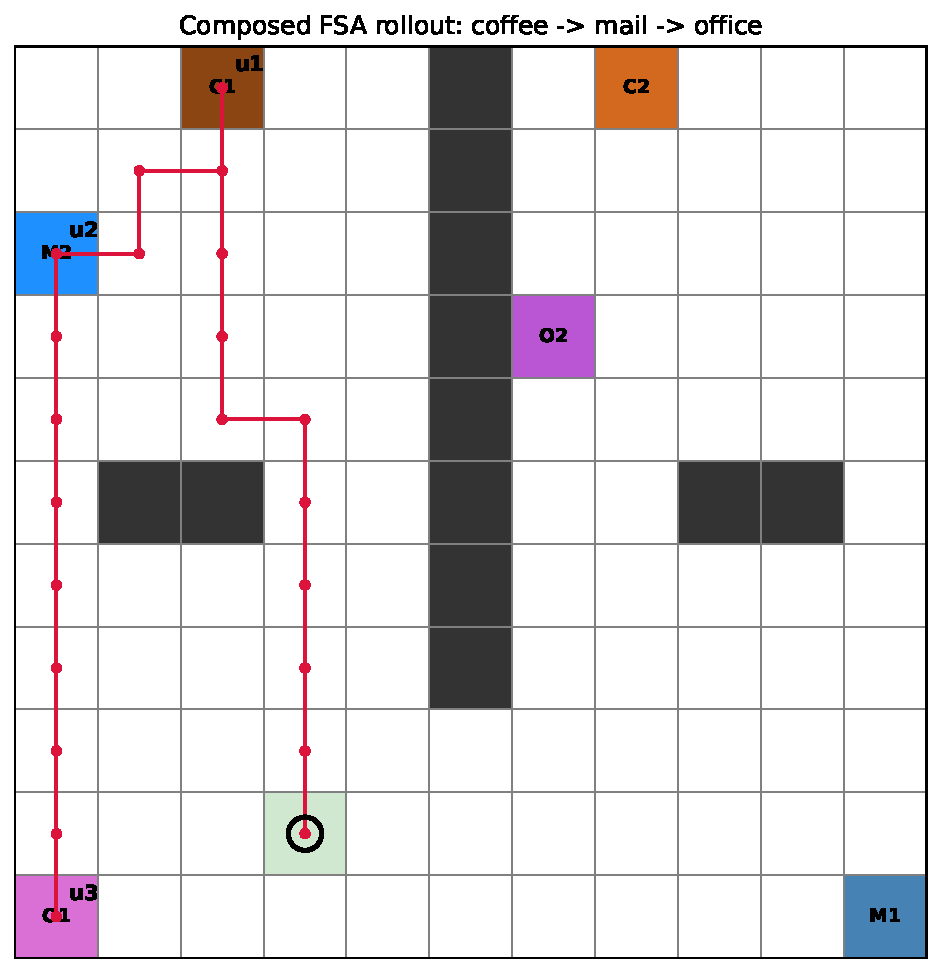
\includegraphics[width=0.7\textwidth]{office_09_fsarollout}
\end{center}

\end{document}
